
\chapter{Overview of neural networks}
\label{neural_networks}

\emph{In this part, a brief introduction is given to NNs, and more specifically, to RBFNNs, which are a special type of these networks. }

From all possible realizations of functions with non-linear behaviour, almost all alternatives can be written in the following basis function formulation, if we assume that the number of basis functions is infinite \cite{norgaard2003neural}

\begin{equation}
\label{basis_NN_eq}
\tilde{y} = \sum_{i = 1}^M w^{(l)}_i \phi_i(u, w^{(nl)}_i).
\end{equation}

The output $\tilde{y}$ is modelled as a weighted sum of $M$ basis functions $\phi_i(\cdot)$.The basis functions are weighted with the linear parameters $w_i$, and they depend on the inputs and set of parameters gathered in $w^{(nl)}_i$. In order to realize a non-linear model, the basis functions need to be some kind of non-linear functions. The parameters of these non-linear functions can take part in the optimization or can be determined priorly. If the latter is the case, linear optimization can be used to find the optimal parameters $w^{(l)}_i$. Therefore, in the further discussion, \eqref{basis_NN_eq} is considered in the form of

 \begin{equation}
\label{basis_NN_eq_lin}
\tilde{y} = \sum_{i = 1}^M w_i \phi_i(u).
\end{equation}

The models in \eqref{basis_NN_eq} and \eqref{basis_NN_eq_lin} are describing NNs. The illustration of an NNs is shown in \figref{fig:nn_example_block}.

\vspace{-5mm}

%Neural network block example 
\begin{figure}[H]
\centering
%
\includegraphics[width=0.35\textwidth]{report/pictures/missingfigure}
\usetikzlibrary{shapes,positioning,matrix}
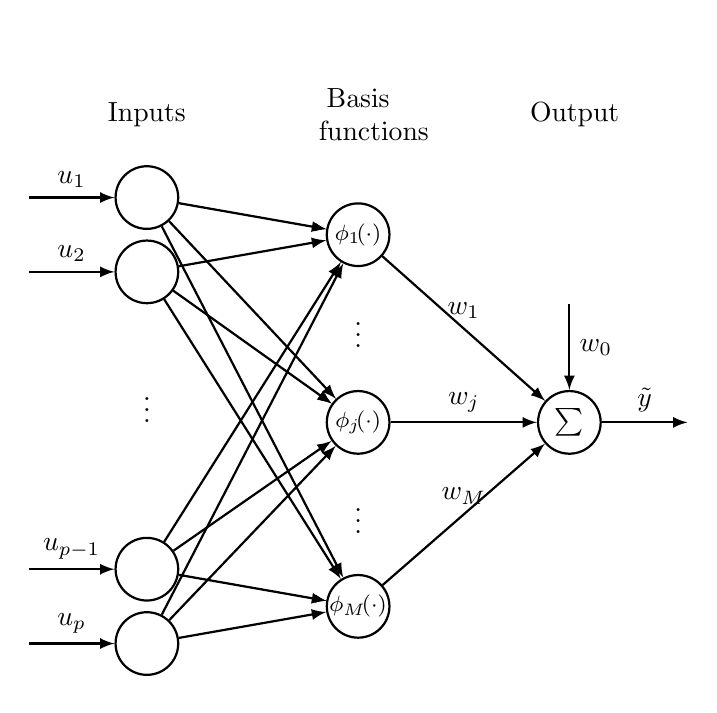
\begin{tikzpicture}[
scale = 1,
plain/.style={
  draw=none,
  fill=none,
  },
net/.style={
  matrix of nodes,
  nodes={
    draw,
    circle,
    thick,
    inner sep=8pt
    },
  nodes in empty cells,
  column sep=0.8cm,
  row sep=-10pt
  },
>=latex
]

\matrix[net] (mat)
{
|[plain]| \parbox{1cm}{\centering Inputs} & 
|[plain]| \parbox{1cm}{\centering Basis\\functions} &
|[plain]| \parbox{1cm}{\centering Output} \\
& |[plain]| \\
|[plain]| & \\
& |[plain]| \\
|[plain]| & |[plain]| $\vdots$ \\
|[plain]| $\vdots$&  &  \\
|[plain]| &  |[plain]|  \\
|[plain]|& |[plain]|$\vdots$ \\
 &  |[plain]|  \\
 |[plain]|&   \\
  &  |[plain]| \\
};

\foreach \ai [count=\mi ]in {2,4}
     \draw[thick][<-] (mat-\ai-1) -- node[above] {$u_\mi$} +(-1.5cm,0);
     \draw[thick][<-] (mat-9-1) -- node[above] {$u_{p-1}$} +(-1.5cm,0);
     \draw[thick][<-] (mat-11-1) -- node[above] {$u_{p}$} +(-1.5cm,0);

\foreach \ai in {2,4,9,11}
{\foreach \aii  in {3,6,10}
  \draw[thick][->] (mat-\ai-1) -- (mat-\aii-2) ;
  
  
}

  \draw[->] (mat-2-1) -- (mat-3-2) node(){\footnotesize $\phi_1\!(\cdot)$};
  \draw [->] (mat-4-1) -- (mat-6-2) node(){\footnotesize$\phi_j\!(\cdot)$};
    \draw [->] (mat-9-1) -- (mat-10-2) node(){\footnotesize$\phi_M\!(\cdot)$};

  \draw[thick][->] (mat-3-2) --node[above]{$w_1$} (mat-6-3)node(){ $\sum$};
  \draw[thick][->] (mat-6-2) --node[above]{$w_j$} (mat-6-3);
  \draw[thick][->] (mat-10-2) --node[above]{$w_M$} (mat-6-3);
  
\draw[thick][->] (mat-6-3) -- node[above] {$\tilde{y}$} +(1.5cm,0);
\draw[thick][<-] (mat-6-3) -- node[right] {$w_0$} +(0,1.5cm);

\end{tikzpicture} 
\caption{Block diagram of a neural network with multiple inputs.}
\label{fig:nn_example_block}
\end{figure}

\vspace{-3mm}

Typically, in literature such as \cite{nelles2013nonlinear, norgaard2003neural}, a NN is distinguished from a non-NN network, when its basis functions are of the same type. In the terminology of NNs, the network in \figref{fig:nn_example_block} is described as follows. The node at the output is called the output neuron, and all output neurons together form the output layer. In the example network, in \figref{fig:nn_example_block}, only one output is considered, therefore the output layer consists of one neuron. The set of $M$ nodes in the center, each of which realizing a basis function, is called the hidden-layer. The inputs are associated with neurons and together they form the input layer. Furthermore, the linear parameters of the network associated with the output neuron(s) are called output weights. The output neuron is usually the linear combination of the basis functions in the hidden layer, with an additional possible offset $w_0$, called the bias. This offset parameter adjusts the operating point. 

The basis functions in the NN formulation are generally multidimensional, defined by the number of inputs. For all NN approaches, however, the multi-variate basis functions are constructed by simple one dimensional functions\cite{nelles2013nonlinear}. This function is called the activation function. Such construction mechanism in the context of NNs is shown in \figref{fig:activation_mechanism}

 %Activation mechanism of NN
\begin{figure}[H]
\centering
%
\includegraphics[width=0.35\textwidth]{report/pictures/missingfigure}
\usetikzlibrary{arrows}
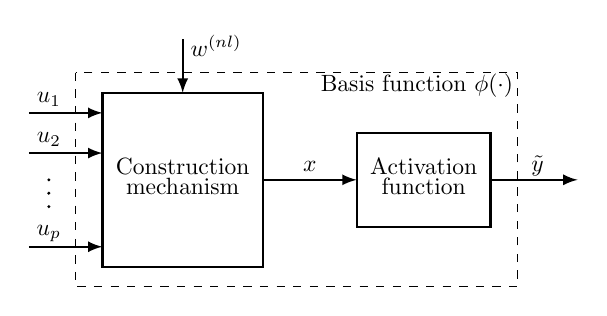
\begin{tikzpicture}[scale=0.85,transform shape]



\draw [thick] (-4.3,3.2) rectangle (-1.9,0.6);
\node at (-3.1,2.1) {Construction};
\node at (-3.1,1.8) {mechanism};
\node at (0.5,2.1) {Activation};
\node at (0.5,1.8) {function};
\draw  [thick] (-0.5,2.6) rectangle (1.5,1.2);
\draw  [thick][-latex](-1.9,1.9) -- (-0.5,1.9);
\node at (-1.2,2.1) {$x$};
\draw [thick] [-latex](1.5,1.9) -- (2.8,1.9);
\node at (2.2,2.1) {$\tilde{y}$};
\draw  [thick][-latex](-5.4,2.9) -- (-4.3,2.9);
\draw  [thick][-latex](-5.4,2.3) -- (-4.3,2.3);
\draw  [thick][-latex](-5.4,0.9) -- (-4.3,0.9);
\node at (-5.1,3.1) {$u_1$};
\node at (-5.1,2.5) {$u_2$};
\node at (-5.1,1.1) {$u_p$};

\node[circle,fill,inner sep=0.5pt] (A) at (-5.1,1.9) {};
\node[circle,fill,inner sep=0.5pt] (A) at (-5.1,1.7) {};
\node[circle,fill,inner sep=0.5pt] (A) at (-5.1,1.5) {};
\draw  [thick][-latex](-3.1,4) -- (-3.1,3.2);
\node at (-2.6,3.9) {$w^{(nl)}$};
\draw [dashed] (-4.7,3.5) rectangle (1.9,0.3);
\node at (0.4,3.3) {Basis function $\phi(\cdot)$};
\end{tikzpicture} 
\caption{Operation of construction mechanism \cite{nelles2013nonlinear}.}
\label{fig:activation_mechanism}
\end{figure}

\vspace{-3mm}

The basis function of the neurons is based on the construction mechanism, that maps the inputs to a scalar $x$ with the help of some non-linear parameters. The activation function then non-linearly transforms the scalar $x$ to the neuron output $\tilde{y}$. 

\subsection{Radial construction}
\label{radial construction}

Among several construction mechanisms, the radial construction is further discussed. In this approach, the scalar $x$ is calculated as the distance between the inputs and the center of the basis functions such that 

 \begin{equation}
\label{radial_structure}
x = ||u- \mu|| = \sqrt{(u-\mu)^T (u-\mu)},
\end{equation}

where $\mu = (\mu_1 \ \mu_2 \ ... \ \mu_M)^T$ is the center vector of the basis functions. The radial construction is utilized for RBF networks, which is discussed in the following sections.


\section{RBF networks}
\label{Radial_basis_function_networks}

 In RBF networks, the first task is to calculate the Euclidean norm, i.e. the distance of the input and center vectors. This is the radial construction mechanism, which is shown in \figref{fig:activation_mechanism}. In the second part, this distance $x$ is transformed by the activation function. Therefore, an RBF network is a class of single hidden layer feedforward networks, expressed as the linear combination of radially symmetric non-linear basis functions \cite{RBF_article}. Typically the choice for the basis functions is the Gaussian function, which is formulated in \eqref{Gaussian_activation} 

\begin{equation}
\label{Gaussian_activation}
\phi(u,\mu_k, \psi_k) = exp \Big(-\frac{||u-\mu_k||^2}{2\psi_k^2}\Big), 
\end{equation}

where $\mu_k \in \: \mathbb{R}^{M}$ determines the center of the RBFs, $\psi_k \in \: \mathbb{R}^{M}$ is the standard deviation of the Gaussian, i.e the width parameter and $||\cdot||$ is the Euclidean norm. Depending on the choice of $\mu$ parameters, the RBFs can overlap each other to capture the information from the input data, while the width parameters $\psi_k$ control the amount of these overlapping basis functions. An example is shown in \figref{fig:rbf_pram}, where the influence of these parameters is illustrated on one RBF neuron, with a single input $u$. 

 %RBFs with different parameters
\begin{figure}[H]
\centering
%
\includegraphics[width=0.35\textwidth]{report/pictures/missingfigure}
% This file was created by matlab2tikz.
%
%The latest updates can be retrieved from
%  http://www.mathworks.com/matlabcentral/fileexchange/22022-matlab2tikz-matlab2tikz
%where you can also make suggestions and rate matlab2tikz.
%
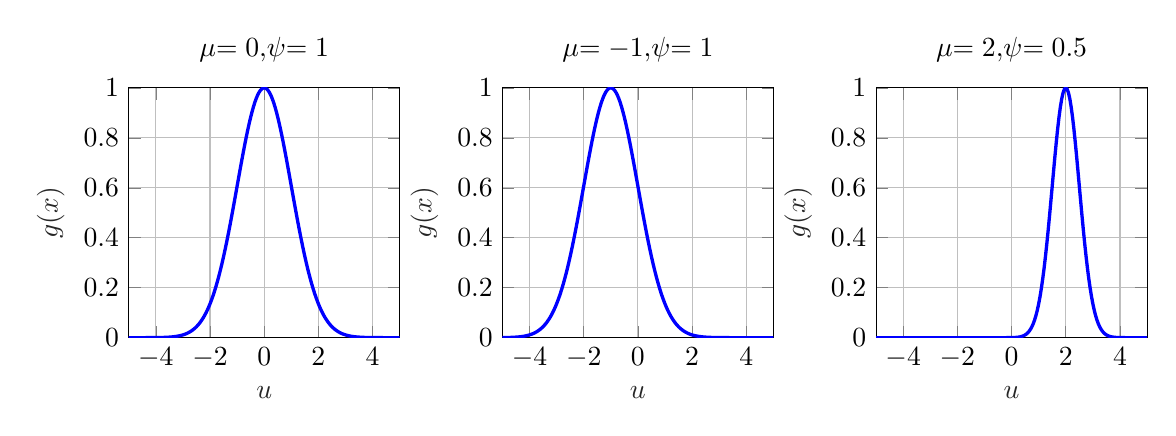
\begin{tikzpicture}

\begin{axis}[%
width=1.355in,
height=1.249in,
at={(1.067in,0.455in)},
scale only axis,
xmin=-5,
xmax=5,
xlabel style={font=\color{white!15!black}},
xlabel={$u$},
ymin=0,
ymax=1,
ylabel style={font=\color{white!15!black}},
ylabel={$g(x)$},
axis background/.style={fill=white},
title style={font=\bfseries},
title={$\mu\text{ = 0, }\psi\text{ = 1}$},
xmajorgrids,
ymajorgrids
]
\addplot [color=blue, line width=1.2pt, forget plot]
  table[row sep=crcr]{%
-5	3.72665317207867e-06\\
-4.95	4.77913973220464e-06\\
-4.9	6.11356796637139e-06\\
-4.85	7.80106730231083e-06\\
-4.8	9.92950430585105e-06\\
-4.75	1.26071051770485e-05\\
-4.7	1.59667838978047e-05\\
-4.65	2.0171295076558e-05\\
-4.6	2.54193465161991e-05\\
-4.55	3.19528237744228e-05\\
-4.5	4.00652973929507e-05\\
-4.45	5.01120028862472e-05\\
-4.4	6.25215037748197e-05\\
-4.35	7.78092686155368e-05\\
-4.3	9.6593413722183e-05\\
-4.25	0.000119612883581023\\
-4.2	0.000147748360232032\\
-4.15	0.000182046210367004\\
-4.1	0.000223745793720617\\
-4.05	0.000274310467493397\\
-4	0.000335462627902507\\
-3.95	0.000409223130228173\\
-3.9	0.000497955421503266\\
-3.85	0.000604414703759546\\
-3.8	0.00073180241888046\\
-3.75	0.000883826306935035\\
-3.7	0.0010647662366679\\
-3.65	0.0012795459378999\\
-3.6	0.00153381067932444\\
-3.55	0.00183401083007313\\
-3.5	0.00218749111818284\\
-3.45	0.00260258525272535\\
-3.4	0.00308871540823671\\
-3.35	0.00365649588005282\\
-3.3	0.00431784000763299\\
-3.25	0.0050860692310126\\
-3.2	0.00597602289500582\\
-3.15	0.00700416714936227\\
-3.1	0.00818870101437391\\
-3.05	0.0095496573950201\\
-3	0.0111089965382421\\
-2.95	0.0128906891440012\\
-2.9	0.0149207860690675\\
-2.85	0.0172274713116347\\
-2.8	0.0198410947443699\\
-2.75	0.0227941808836118\\
-2.7	0.0261214098539177\\
-2.65	0.0298595666411149\\
-2.6	0.0340474547345986\\
-2.55	0.0387257703516635\\
-2.5	0.0439369336234064\\
-2.45	0.0497248734123485\\
-2.4	0.0561347628341325\\
-2.35	0.0632127030752875\\
-2.3	0.0710053537396354\\
-2.25	0.0795595087182259\\
-2.2	0.0889216174593844\\
-2.15	0.0991372525107452\\
-2.1	0.110250525304483\\
-2.05	0.122303453346898\\
-2	0.13533528323661\\
-1.95	0.149381775250415\\
-1.9	0.164474456577152\\
-1.85	0.18063985161889\\
-1.8	0.197898699083611\\
-1.75	0.216265166829883\\
-1.7	0.235746076555859\\
-1.65	0.256340151415069\\
-1.6	0.27803730045319\\
-1.55	0.300817954357271\\
-1.5	0.324652467358345\\
-1.45	0.349500600199751\\
-1.4	0.375311098851394\\
-1.35	0.402021383094649\\
-1.3	0.429557358210734\\
-1.25	0.457833361771608\\
-1.2	0.486752255959966\\
-1.15	0.51620567394549\\
-1.1	0.546074426639704\\
-1.05	0.576229073671794\\
-1	0.606530659712628\\
-0.95	0.636831614371737\\
-0.899999999999999	0.666976810858469\\
-0.85	0.696804775496029\\
-0.8	0.726149037073685\\
-0.75	0.754839601989002\\
-0.7	0.782704538241863\\
-0.649999999999999	0.809571648667882\\
-0.6	0.835270211411267\\
-0.55	0.859632763602538\\
-0.5	0.882496902584591\\
-0.45	0.903707077873192\\
-0.399999999999999	0.923116346386632\\
-0.35	0.940588063364339\\
-0.3	0.955997481833097\\
-0.25	0.969233234476342\\
-0.199999999999999	0.980198673306753\\
-0.149999999999999	0.988813044611232\\
-0.0999999999999996	0.995012479192681\\
-0.0499999999999998	0.99875078092458\\
0	1\\
0.0499999999999998	0.998750780924581\\
0.0999999999999996	0.995012479192683\\
0.149999999999999	0.988813044611234\\
0.199999999999999	0.980198673306757\\
0.25	0.969233234476346\\
0.3	0.955997481833103\\
0.35	0.940588063364345\\
0.399999999999999	0.923116346386639\\
0.45	0.9037070778732\\
0.5	0.8824969025846\\
0.55	0.859632763602547\\
0.6	0.835270211411277\\
0.649999999999999	0.809571648667892\\
0.7	0.782704538241873\\
0.75	0.754839601989013\\
0.8	0.726149037073696\\
0.85	0.69680477549604\\
0.899999999999999	0.66697681085848\\
0.95	0.636831614371749\\
1	0.606530659712639\\
1.05	0.576229073671805\\
1.1	0.546074426639715\\
1.15	0.516205673945502\\
1.2	0.486752255959977\\
1.25	0.457833361771619\\
1.3	0.429557358210744\\
1.35	0.40202138309466\\
1.4	0.375311098851404\\
1.45	0.349500600199761\\
1.5	0.324652467358354\\
1.55	0.30081795435728\\
1.6	0.278037300453198\\
1.65	0.256340151415077\\
1.7	0.235746076555867\\
1.75	0.21626516682989\\
1.8	0.197898699083618\\
1.85	0.180639851618897\\
1.9	0.164474456577157\\
1.95	0.14938177525042\\
2	0.135335283236615\\
2.05	0.122303453346903\\
2.1	0.110250525304487\\
2.15	0.0991372525107492\\
2.2	0.088921617459388\\
2.25	0.0795595087182293\\
2.3	0.0710053537396385\\
2.35	0.0632127030752902\\
2.4	0.056134762834135\\
2.45	0.0497248734123508\\
2.5	0.0439369336234085\\
2.55	0.0387257703516653\\
2.6	0.0340474547346002\\
2.65	0.0298595666411163\\
2.7	0.026121409853919\\
2.75	0.022794180883613\\
2.8	0.0198410947443709\\
2.85	0.0172274713116357\\
2.9	0.0149207860690683\\
2.95	0.0128906891440019\\
3	0.0111089965382427\\
3.05	0.00954965739502065\\
3.1	0.00818870101437438\\
3.15	0.00700416714936269\\
3.2	0.00597602289500618\\
3.25	0.0050860692310129\\
3.3	0.00431784000763326\\
3.35	0.00365649588005305\\
3.4	0.00308871540823691\\
3.45	0.00260258525272552\\
3.5	0.00218749111818299\\
3.55	0.00183401083007325\\
3.6	0.00153381067932454\\
3.65	0.00127954593789999\\
3.7	0.00106476623666798\\
3.75	0.000883826306935097\\
3.8	0.000731802418880512\\
3.85	0.000604414703759589\\
3.9	0.000497955421503302\\
3.95	0.000409223130228203\\
4	0.000335462627902532\\
4.05	0.000274310467493418\\
4.1	0.000223745793720634\\
4.15	0.000182046210367018\\
4.2	0.000147748360232044\\
4.25	0.000119612883581032\\
4.3	9.65934137221907e-05\\
4.35	7.78092686155432e-05\\
4.4	6.25215037748248e-05\\
4.45	5.01120028862513e-05\\
4.5	4.00652973929541e-05\\
4.55	3.19528237744255e-05\\
4.6	2.54193465162013e-05\\
4.65	2.01712950765598e-05\\
4.7	1.59667838978061e-05\\
4.75	1.26071051770496e-05\\
4.8	9.92950430585193e-06\\
4.85	7.80106730231153e-06\\
4.9	6.11356796637196e-06\\
4.95	4.77913973220508e-06\\
5	3.72665317207902e-06\\
};
\end{axis}

\begin{axis}[%
xshift=-0.7cm,
width=1.355in,
height=1.249in,
at={(3.211in,0.455in)},
scale only axis,
xmin=-5,
xmax=5,
xlabel style={font=\color{white!15!black}},
xlabel={$u$},
ymin=0,
ymax=1,
ylabel style={font=\color{white!15!black}},
ylabel={$g(x)$},
axis background/.style={fill=white},
title style={font=\bfseries},
title={$\mu\text{ = -1, }\psi\text{ = 1}$},
xmajorgrids,
ymajorgrids
]
\addplot [color=blue, line width=1.2pt, forget plot]
  table[row sep=crcr]{%
-5	0.000335462627902512\\
-4.95	0.000409223130228179\\
-4.9	0.000497955421503273\\
-4.85	0.000604414703759554\\
-4.8	0.000731802418880471\\
-4.75	0.000883826306935047\\
-4.7	0.00106476623666792\\
-4.65	0.00127954593789992\\
-4.6	0.00153381067932446\\
-4.55	0.00183401083007315\\
-4.5	0.00218749111818287\\
-4.45	0.00260258525272538\\
-4.4	0.00308871540823675\\
-4.35	0.00365649588005287\\
-4.3	0.00431784000763304\\
-4.25	0.00508606923101266\\
-4.2	0.00597602289500589\\
-4.15	0.00700416714936235\\
-4.1	0.008188701014374\\
-4.05	0.00954965739502021\\
-4	0.0111089965382422\\
-3.95	0.0128906891440013\\
-3.9	0.0149207860690677\\
-3.85	0.0172274713116349\\
-3.8	0.01984109474437\\
-3.75	0.0227941808836121\\
-3.7	0.0261214098539179\\
-3.65	0.0298595666411151\\
-3.6	0.0340474547345989\\
-3.55	0.0387257703516639\\
-3.5	0.0439369336234068\\
-3.45	0.0497248734123489\\
-3.4	0.056134762834133\\
-3.35	0.063212703075288\\
-3.3	0.071005353739636\\
-3.25	0.0795595087182265\\
-3.2	0.0889216174593851\\
-3.15	0.099137252510746\\
-3.1	0.110250525304484\\
-3.05	0.122303453346899\\
-3	0.135335283236611\\
-2.95	0.149381775250416\\
-2.9	0.164474456577153\\
-2.85	0.180639851618891\\
-2.8	0.197898699083612\\
-2.75	0.216265166829884\\
-2.7	0.23574607655586\\
-2.65	0.25634015141507\\
-2.6	0.27803730045319\\
-2.55	0.300817954357271\\
-2.5	0.324652467358345\\
-2.45	0.349500600199752\\
-2.4	0.375311098851395\\
-2.35	0.40202138309465\\
-2.3	0.429557358210734\\
-2.25	0.457833361771609\\
-2.2	0.486752255959966\\
-2.15	0.51620567394549\\
-2.1	0.546074426639703\\
-2.05	0.576229073671794\\
-2	0.606530659712627\\
-1.95	0.636831614371737\\
-1.9	0.666976810858468\\
-1.85	0.696804775496028\\
-1.8	0.726149037073685\\
-1.75	0.754839601989001\\
-1.7	0.782704538241862\\
-1.65	0.809571648667881\\
-1.6	0.835270211411267\\
-1.55	0.859632763602537\\
-1.5	0.882496902584591\\
-1.45	0.903707077873192\\
-1.4	0.923116346386632\\
-1.35	0.940588063364339\\
-1.3	0.955997481833097\\
-1.25	0.969233234476342\\
-1.2	0.980198673306753\\
-1.15	0.988813044611232\\
-1.1	0.995012479192681\\
-1.05	0.99875078092458\\
-1	1\\
-0.95	0.998750780924581\\
-0.899999999999999	0.995012479192683\\
-0.85	0.988813044611234\\
-0.8	0.980198673306757\\
-0.75	0.969233234476346\\
-0.7	0.955997481833103\\
-0.649999999999999	0.940588063364345\\
-0.6	0.923116346386639\\
-0.55	0.9037070778732\\
-0.5	0.8824969025846\\
-0.45	0.859632763602547\\
-0.399999999999999	0.835270211411277\\
-0.35	0.809571648667892\\
-0.3	0.782704538241873\\
-0.25	0.754839601989013\\
-0.199999999999999	0.726149037073696\\
-0.149999999999999	0.69680477549604\\
-0.0999999999999996	0.66697681085848\\
-0.0499999999999998	0.636831614371749\\
0	0.606530659712639\\
0.0499999999999998	0.576229073671806\\
0.0999999999999996	0.546074426639715\\
0.149999999999999	0.516205673945502\\
0.199999999999999	0.486752255959977\\
0.25	0.45783336177162\\
0.3	0.429557358210744\\
0.35	0.40202138309466\\
0.399999999999999	0.375311098851405\\
0.45	0.349500600199761\\
0.5	0.324652467358354\\
0.55	0.30081795435728\\
0.6	0.278037300453198\\
0.649999999999999	0.256340151415078\\
0.7	0.235746076555867\\
0.75	0.216265166829891\\
0.8	0.197898699083618\\
0.85	0.180639851618897\\
0.899999999999999	0.164474456577158\\
0.95	0.149381775250421\\
1	0.135335283236615\\
1.05	0.122303453346903\\
1.1	0.110250525304487\\
1.15	0.0991372525107493\\
1.2	0.088921617459388\\
1.25	0.0795595087182293\\
1.3	0.0710053537396385\\
1.35	0.0632127030752901\\
1.4	0.0561347628341349\\
1.45	0.0497248734123507\\
1.5	0.0439369336234084\\
1.55	0.0387257703516652\\
1.6	0.0340474547346001\\
1.65	0.0298595666411162\\
1.7	0.0261214098539189\\
1.75	0.0227941808836129\\
1.8	0.0198410947443707\\
1.85	0.0172274713116355\\
1.9	0.0149207860690682\\
1.95	0.0128906891440018\\
2	0.0111089965382426\\
2.05	0.00954965739502055\\
2.1	0.00818870101437429\\
2.15	0.00700416714936261\\
2.2	0.00597602289500611\\
2.25	0.00508606923101284\\
2.3	0.00431784000763321\\
2.35	0.00365649588005301\\
2.4	0.00308871540823687\\
2.45	0.00260258525272549\\
2.5	0.00218749111818296\\
2.55	0.00183401083007322\\
2.6	0.00153381067932452\\
2.65	0.00127954593789997\\
2.7	0.00106476623666796\\
2.75	0.000883826306935085\\
2.8	0.000731802418880503\\
2.85	0.000604414703759581\\
2.9	0.000497955421503296\\
2.95	0.000409223130228197\\
3	0.000335462627902527\\
3.05	0.000274310467493414\\
3.1	0.000223745793720631\\
3.15	0.000182046210367015\\
3.2	0.000147748360232041\\
3.25	0.000119612883581031\\
3.3	9.65934137221892e-05\\
3.35	7.78092686155419e-05\\
3.4	6.25215037748238e-05\\
3.45	5.01120028862505e-05\\
3.5	4.00652973929535e-05\\
3.55	3.1952823774425e-05\\
3.6	2.54193465162008e-05\\
3.65	2.01712950765595e-05\\
3.7	1.59667838978058e-05\\
3.75	1.26071051770494e-05\\
3.8	9.92950430585177e-06\\
3.85	7.80106730231139e-06\\
3.9	6.11356796637185e-06\\
3.95	4.77913973220499e-06\\
4	3.72665317207895e-06\\
4.05	2.89869477463316e-06\\
4.1	2.24905596703252e-06\\
4.15	1.74065339649344e-06\\
4.2	1.34381227763163e-06\\
4.25	1.03485421110946e-06\\
4.3	7.94939361534982e-07\\
4.35	6.09120331551606e-07\\
4.4	4.6557157157835e-07\\
4.45	3.54963808697164e-07\\
4.5	2.69957850336326e-07\\
4.55	2.04796302119765e-07\\
4.6	1.54975313570305e-07\\
4.65	1.1698150401353e-07\\
4.7	8.80817919646143e-08\\
4.75	6.61560163769838e-08\\
4.8	4.95640531917301e-08\\
4.85	3.70406455079473e-08\\
4.9	2.76124245682834e-08\\
4.95	2.05326404492339e-08\\
5	1.52299797447143e-08\\
};
\end{axis}

\begin{axis}[%
xshift=-1.4cm,
width=1.355in,
height=1.249in,
at={(5.355in,0.455in)},
scale only axis,
xmin=-5,
xmax=5,
xlabel style={font=\color{white!15!black}},
xlabel={$u$},
ymin=0,
ymax=1,
ylabel style={font=\color{white!15!black}},
ylabel={$g(x)$},
axis background/.style={fill=white},
title style={font=\bfseries},
title={$\mu\text{ = 2, }\psi\text{ = 0.5}$},
xmajorgrids,
ymajorgrids
]
\addplot [color=blue, line width=1.2pt, forget plot]
  table[row sep=crcr]{%
-5	2.74878500791021e-43\\
-4.95	1.10912776125503e-42\\
-4.9	4.43077231241282e-42\\
-4.85	1.75240444373849e-41\\
-4.8	6.86193047676127e-41\\
-4.75	2.66020641594391e-40\\
-4.7	1.02103684608935e-39\\
-4.65	3.87993587628423e-39\\
-4.6	1.45970379320953e-38\\
-4.55	5.43703314193213e-38\\
-4.5	2.00500878196157e-37\\
-4.45	7.32027899105949e-37\\
-4.4	2.64603779068747e-36\\
-4.35	9.46937917271538e-36\\
-4.3	3.35508885623091e-35\\
-4.25	1.17691094392159e-34\\
-4.2	4.08733497286565e-34\\
-4.15	1.40538047776279e-33\\
-4.1	4.7841485558165e-33\\
-4.05	1.6123987480501e-32\\
-4	5.38018616002068e-32\\
-3.95	1.77737557956817e-31\\
-3.9	5.81323888488905e-31\\
-3.85	1.88240984759479e-30\\
-3.8	6.03486080597041e-30\\
-3.75	1.91547895196696e-29\\
-3.7	6.01928027681589e-29\\
-3.65	1.87270255445602e-28\\
-3.6	5.76832996124723e-28\\
-3.55	1.75909154968455e-27\\
-3.5	5.31109224967845e-27\\
-3.45	1.58758249826435e-26\\
-3.4	4.69835486089745e-26\\
-3.35	1.37661463866175e-25\\
-3.3	3.99333740985715e-25\\
-3.25	1.14687658222545e-24\\
-3.2	3.26102718071061e-24\\
-3.15	9.18013795095797e-24\\
-3.1	2.55859208104832e-23\\
-3.05	7.06008533726155e-23\\
-3	1.92874984796364e-22\\
-2.95	5.2167366620263e-22\\
-2.9	1.3969439431469e-21\\
-2.85	3.70353197765179e-21\\
-2.8	9.72098502029933e-21\\
-2.75	2.52616378092532e-20\\
-2.7	6.49934797206988e-20\\
-2.65	1.65552266209852e-19\\
-2.6	4.17501005584986e-19\\
-2.55	1.04240617839e-18\\
-2.5	2.57675710915456e-18\\
-2.45	6.30618989398542e-18\\
-2.4	1.52797996828705e-17\\
-2.35	3.66543339560045e-17\\
-2.3	8.70542662229477e-17\\
-2.25	2.04697171316387e-16\\
-2.2	4.76530473529831e-16\\
-2.15	1.09831412982841e-15\\
-2.1	2.50622188714485e-15\\
-2.05	5.66199551694798e-15\\
-2	1.2664165549092e-14\\
-1.95	2.80440473822231e-14\\
-1.9	6.14839641270375e-14\\
-1.85	1.33456608482178e-13\\
-1.8	2.86797500888764e-13\\
-1.75	6.10193667760435e-13\\
-1.7	1.28533722513345e-12\\
-1.65	2.68054763731221e-12\\
-1.6	5.53461007170021e-12\\
-1.55	1.13137762000636e-11\\
-1.5	2.28973484564523e-11\\
-1.45	4.58796248713866e-11\\
-1.4	9.10147076448671e-11\\
-1.35	1.78755887112773e-10\\
-1.3	3.47589128123947e-10\\
-1.25	6.69158609129193e-10\\
-1.2	1.27540762952588e-09\\
-1.15	2.40672243630074e-09\\
-1.1	4.49634946228031e-09\\
-1.05	8.31670245682736e-09\\
-1	1.52299797447108e-08\\
-0.95	2.76124245682771e-08\\
-0.899999999999999	4.95640531917193e-08\\
-0.85	8.80817919645962e-08\\
-0.8	1.54975313570273e-07\\
-0.75	2.69957850336272e-07\\
-0.7	4.65571571578261e-07\\
-0.649999999999999	7.94939361534836e-07\\
-0.6	1.34381227763139e-06\\
-0.55	2.24905596703212e-06\\
-0.5	3.72665317207832e-06\\
-0.45	6.11356796637084e-06\\
-0.399999999999999	9.9295043058502e-06\\
-0.35	1.59667838978033e-05\\
-0.3	2.5419346516197e-05\\
-0.25	4.00652973929477e-05\\
-0.199999999999999	6.2521503774815e-05\\
-0.149999999999999	9.65934137221763e-05\\
-0.0999999999999996	0.000147748360232022\\
-0.0499999999999998	0.000223745793720603\\
0	0.000335462627902487\\
0.0499999999999998	0.000497955421503237\\
0.0999999999999996	0.00073180241888042\\
0.149999999999999	0.00106476623666785\\
0.199999999999999	0.00153381067932436\\
0.25	0.00218749111818274\\
0.3	0.00308871540823657\\
0.35	0.00431784000763281\\
0.399999999999999	0.00597602289500558\\
0.45	0.0081887010143736\\
0.5	0.0111089965382417\\
0.55	0.014920786069067\\
0.6	0.0198410947443693\\
0.649999999999999	0.0261214098539169\\
0.7	0.0340474547345977\\
0.75	0.0439369336234054\\
0.8	0.0561347628341313\\
0.85	0.0710053537396339\\
0.899999999999999	0.0889216174593828\\
0.95	0.110250525304481\\
1	0.135335283236608\\
1.05	0.164474456577149\\
1.1	0.197898699083608\\
1.15	0.235746076555856\\
1.2	0.278037300453186\\
1.25	0.324652467358341\\
1.3	0.37531109885139\\
1.35	0.429557358210729\\
1.4	0.486752255959961\\
1.45	0.546074426639699\\
1.5	0.606530659712623\\
1.55	0.666976810858464\\
1.6	0.726149037073681\\
1.65	0.782704538241859\\
1.7	0.835270211411264\\
1.75	0.882496902584588\\
1.8	0.92311634638663\\
1.85	0.955997481833095\\
1.9	0.980198673306752\\
1.95	0.995012479192681\\
2	1\\
2.05	0.995012479192684\\
2.1	0.980198673306759\\
2.15	0.955997481833105\\
2.2	0.923116346386642\\
2.25	0.882496902584603\\
2.3	0.835270211411281\\
2.35	0.782704538241878\\
2.4	0.726149037073702\\
2.45	0.666976810858486\\
2.5	0.606530659712645\\
2.55	0.546074426639721\\
2.6	0.486752255959984\\
2.65	0.429557358210751\\
2.7	0.375311098851411\\
2.75	0.32465246735836\\
2.8	0.278037300453204\\
2.85	0.235746076555872\\
2.9	0.197898699083623\\
2.95	0.164474456577162\\
3	0.135335283236619\\
3.05	0.110250525304491\\
3.1	0.088921617459391\\
3.15	0.0710053537396409\\
3.2	0.056134762834137\\
3.25	0.0439369336234101\\
3.3	0.0340474547346016\\
3.35	0.02612140985392\\
3.4	0.0198410947443717\\
3.45	0.014920786069069\\
3.5	0.0111089965382432\\
3.55	0.00818870101437477\\
3.6	0.00597602289500647\\
3.65	0.00431784000763347\\
3.7	0.00308871540823707\\
3.75	0.0021874911181831\\
3.8	0.00153381067932462\\
3.85	0.00106476623666804\\
3.9	0.000731802418880555\\
3.95	0.000497955421503332\\
4	0.000335462627902552\\
4.05	0.000223745793720648\\
4.1	0.000147748360232053\\
4.15	9.65934137221969e-05\\
4.2	6.25215037748289e-05\\
4.25	4.00652973929568e-05\\
4.3	2.5419346516203e-05\\
4.35	1.59667838978072e-05\\
4.4	9.92950430585265e-06\\
4.45	6.11356796637241e-06\\
4.5	3.7266531720793e-06\\
4.55	2.24905596703273e-06\\
4.6	1.34381227763176e-06\\
4.65	7.94939361535061e-07\\
4.7	4.65571571578397e-07\\
4.75	2.69957850336354e-07\\
4.8	1.54975313570321e-07\\
4.85	8.80817919646237e-08\\
4.9	4.95640531917355e-08\\
4.95	2.76124245682864e-08\\
5	1.5229979744716e-08\\
};
\end{axis}
\end{tikzpicture}% 
\caption{The width and the position of the Gaussian basis function in terms of $\psi$ and $\mu$.}
\label{fig:rbf_pram}
\end{figure}

\vspace{-3mm}

Therefore, when an RBF network is chosen for identification, three types of parameters need to be considered. The output weights $w_i$ are linear parameters. They define the heights of the basis functions and the bias, i.e the offset value. The centers $\mu$ are non-linear parameters of the hidden layer neurons. They determine the positions of the basis functions. Furthermore, the standard deviations $\psi$ are also non-linear parameters of the hidden-layer neurons. During the optimization, these parameters have to be somehow determined and optimized. \figref{fig:rbf_interpol} illustrates the interpolation capability of RBF networks. 

 %Interpolation of RBFS
\begin{figure}[H]
\centering
%
\includegraphics[width=0.35\textwidth]{report/pictures/missingfigure}
% This file was created by matlab2tikz.
%
%The latest updates can be retrieved from
%  http://www.mathworks.com/matlabcentral/fileexchange/22022-matlab2tikz-matlab2tikz
%where you can also make suggestions and rate matlab2tikz.
%
\definecolor{mycolor1}{rgb}{0.00000,0.44700,0.74100}%
\definecolor{mycolor2}{rgb}{0.85000,0.32500,0.09800}%
\definecolor{mycolor3}{rgb}{0.92900,0.69400,0.12500}%
%
\begin{tikzpicture}

\begin{axis}[%
width=2.274in,
height=1.182in,
at={(1.039in,0.43in)},
scale only axis,
xmin=-4,
xmax=4,
xlabel style={font=\color{white!15!black}},
xlabel={x},
ymin=-4,
ymax=10,
ylabel style={font=\color{white!15!black}},
ylabel={y(x)},
axis background/.style={fill=white},
title style={font=\bfseries},
title={$y = x(x+1.5)(x-1.5)(x-2)$}
]
\addplot[const plot, color=blue, line width=1.2pt, forget plot] table[row sep=crcr] {%
-4	330\\
-3.99	326.71675701\\
-3.98	323.45695616\\
-3.97	320.22048981\\
-3.96	317.00725056\\
-3.95	313.81713125\\
-3.94	310.65002496\\
-3.93	307.50582501\\
-3.92	304.38442496\\
-3.91	301.28571861\\
-3.9	298.2096\\
-3.89	295.15596341\\
-3.88	292.12470336\\
-3.87	289.11571461\\
-3.86	286.12889216\\
-3.85	283.16413125\\
-3.84	280.22132736\\
-3.83	277.30037621\\
-3.82	274.40117376\\
-3.81	271.52361621\\
-3.8	268.6676\\
-3.79	265.83302181\\
-3.78	263.01977856\\
-3.77	260.22776741\\
-3.76	257.45688576\\
-3.75	254.70703125\\
-3.74	251.97810176\\
-3.73	249.26999541\\
-3.72	246.58261056\\
-3.71	243.91584581\\
-3.7	241.2696\\
-3.69	238.64377221\\
-3.68	236.03826176\\
-3.67	233.45296821\\
-3.66	230.88779136\\
-3.65	228.34263125\\
-3.64	225.81738816\\
-3.63	223.31196261\\
-3.62	220.82625536\\
-3.61	218.36016741\\
-3.6	215.9136\\
-3.59	213.48645461\\
-3.58	211.07863296\\
-3.57	208.69003701\\
-3.56	206.32056896\\
-3.55	203.97013125\\
-3.54	201.63862656\\
-3.53	199.32595781\\
-3.52	197.03202816\\
-3.51	194.75674101\\
-3.5	192.5\\
-3.49	190.26170901\\
-3.48	188.04177216\\
-3.47	185.84009381\\
-3.46	183.65657856\\
-3.45	181.49113125\\
-3.44	179.34365696\\
-3.43	177.21406101\\
-3.42	175.10224896\\
-3.41	173.00812661\\
-3.4	170.9316\\
-3.39	168.87257541\\
-3.38	166.83095936\\
-3.37	164.80665861\\
-3.36	162.79958016\\
-3.35	160.80963125\\
-3.34	158.83671936\\
-3.33	156.88075221\\
-3.32	154.94163776\\
-3.31	153.01928421\\
-3.3	151.1136\\
-3.29	149.22449381\\
-3.28	147.35187456\\
-3.27	145.49565141\\
-3.26	143.65573376\\
-3.25	141.83203125\\
-3.24	140.02445376\\
-3.23	138.23291141\\
-3.22	136.45731456\\
-3.21	134.69757381\\
-3.2	132.9536\\
-3.19	131.22530421\\
-3.18	129.51259776\\
-3.17	127.81539221\\
-3.16	126.13359936\\
-3.15	124.46713125\\
-3.14	122.81590016\\
-3.13	121.17981861\\
-3.12	119.55879936\\
-3.11	117.95275541\\
-3.1	116.3616\\
-3.09	114.78524661\\
-3.08	113.22360896\\
-3.07	111.67660101\\
-3.06	110.14413696\\
-3.05	108.62613125\\
-3.04	107.12249856\\
-3.03	105.63315381\\
-3.02	104.15801216\\
-3.01	102.69698901\\
-3	101.25\\
-2.99	99.81696101\\
-2.98	98.39778816\\
-2.97	96.99239781\\
-2.96	95.60070656\\
-2.95	94.22263125\\
-2.94	92.85808896\\
-2.93	91.50699701\\
-2.92	90.16927296\\
-2.91	88.84483461\\
-2.9	87.5336\\
-2.89	86.2354874099999\\
-2.88	84.95041536\\
-2.87	83.67830261\\
-2.86	82.41906816\\
-2.85	81.17263125\\
-2.84	79.93891136\\
-2.83	78.71782821\\
-2.82	77.50930176\\
-2.81	76.31325221\\
-2.8	75.1296\\
-2.79	73.95826581\\
-2.78	72.79917056\\
-2.77	71.65223541\\
-2.76	70.51738176\\
-2.75	69.39453125\\
-2.74	68.28360576\\
-2.73	67.18452741\\
-2.72	66.09721856\\
-2.71	65.02160181\\
-2.7	63.9576\\
-2.69	62.90513621\\
-2.68	61.86413376\\
-2.67	60.83451621\\
-2.66	59.81620736\\
-2.65	58.80913125\\
-2.64	57.81321216\\
-2.63	56.82837461\\
-2.62	55.85454336\\
-2.61	54.89164341\\
-2.6	53.9396\\
-2.59	52.99833861\\
-2.58	52.06778496\\
-2.57	51.14786501\\
-2.56	50.23850496\\
-2.55	49.33963125\\
-2.54	48.45117056\\
-2.53	47.57304981\\
-2.52	46.70519616\\
-2.51	45.84753701\\
-2.5	45\\
-2.49	44.16251301\\
-2.48	43.33500416\\
-2.47	42.51740181\\
-2.46	41.70963456\\
-2.45	40.91163125\\
-2.44	40.12332096\\
-2.43	39.34463301\\
-2.42	38.57549696\\
-2.41	37.81584261\\
-2.4	37.0656\\
-2.39	36.32469941\\
-2.38	35.59307136\\
-2.37	34.87064661\\
-2.36	34.15735616\\
-2.35	33.45313125\\
-2.34	32.75790336\\
-2.33	32.07160421\\
-2.32	31.39416576\\
-2.31	30.72552021\\
-2.3	30.0656\\
-2.29	29.41433781\\
-2.28	28.77166656\\
-2.27	28.13751941\\
-2.26	27.51182976\\
-2.25	26.89453125\\
-2.24	26.28555776\\
-2.23	25.68484341\\
-2.22	25.09232256\\
-2.21	24.50792981\\
-2.2	23.9316\\
-2.19	23.36326821\\
-2.18	22.80286976\\
-2.17	22.25034021\\
-2.16	21.70561536\\
-2.15	21.16863125\\
-2.14	20.63932416\\
-2.13	20.11763061\\
-2.12	19.60348736\\
-2.11	19.09683141\\
-2.1	18.5976\\
-2.09	18.10573061\\
-2.08	17.62116096\\
-2.07	17.14382901\\
-2.06	16.67367296\\
-2.05	16.21063125\\
-2.04	15.75464256\\
-2.03	15.30564581\\
-2.02	14.86358016\\
-2.01	14.42838501\\
-2	14\\
-1.99	13.57836501\\
-1.98	13.16342016\\
-1.97	12.75510581\\
-1.96	12.35336256\\
-1.95	11.95813125\\
-1.94	11.56935296\\
-1.93	11.18696901\\
-1.92	10.81092096\\
-1.91	10.44115061\\
-1.9	10.0776\\
-1.89	9.72021141\\
-1.88	9.36892736\\
-1.87	9.02369061\\
-1.86	8.68444416\\
-1.85	8.35113125\\
-1.84	8.02369536\\
-1.83	7.70208021\\
-1.82	7.38622976\\
-1.81	7.07608821\\
-1.8	6.77159999999999\\
-1.79	6.47270981\\
-1.78	6.17936255999999\\
-1.77	5.89150341\\
-1.76	5.60907775999999\\
-1.75	5.33203125\\
-1.74	5.06030975999999\\
-1.73	4.79385941\\
-1.72	4.53262655999999\\
-1.71	4.27655781\\
-1.7	4.02559999999999\\
-1.69	3.77970021\\
-1.68	3.53880576\\
-1.67	3.30286421\\
-1.66	3.07182336\\
-1.65	2.84563125\\
-1.64	2.62423616\\
-1.63	2.40758661\\
-1.62	2.19563136\\
-1.61	1.98831941\\
-1.6	1.7856\\
-1.59	1.58742261\\
-1.58	1.39373696\\
-1.57	1.20449301\\
-1.56	1.01964096\\
-1.55	0.839131249999997\\
-1.54	0.662914560000001\\
-1.53	0.490941809999997\\
-1.52	0.32316416\\
-1.51	0.159533009999997\\
-1.5	-0\\
-1.49	-0.155482990000004\\
-1.48	-0.30696384\\
-1.47	-0.454490190000004\\
-1.46	-0.598109440000001\\
-1.45	-0.737868750000004\\
-1.44	-0.873815040000001\\
-1.43	-1.00599499\\
-1.42	-1.13445504\\
-1.41	-1.25924139\\
-1.4	-1.3804\\
-1.39	-1.49797659\\
-1.38	-1.61201664\\
-1.37	-1.72256539\\
-1.36	-1.82966784\\
-1.35	-1.93336875\\
-1.34	-2.03371264\\
-1.33	-2.13074379\\
-1.32	-2.22450624\\
-1.31	-2.31504379\\
-1.3	-2.4024\\
-1.29	-2.48661819\\
-1.28	-2.56774144\\
-1.27	-2.64581259\\
-1.26	-2.72087424\\
-1.25	-2.79296875\\
-1.24	-2.86213824\\
-1.23	-2.92842459\\
-1.22	-2.99186944\\
-1.21	-3.05251419\\
-1.2	-3.1104\\
-1.19	-3.16556779\\
-1.18	-3.21805824\\
-1.17	-3.26791179\\
-1.16	-3.31516864\\
-1.15	-3.35986875\\
-1.14	-3.40205184\\
-1.13	-3.44175739\\
-1.12	-3.47902464\\
-1.11	-3.51389259\\
-1.1	-3.5464\\
-1.09	-3.57658539\\
-1.08	-3.60448704\\
-1.07	-3.63014299\\
-1.06	-3.65359104\\
-1.05	-3.67486875\\
-1.04	-3.69401344\\
-1.03	-3.71106219\\
-1.02	-3.72605184\\
-1.01	-3.73901899\\
-1	-3.75\\
-0.99	-3.75903099\\
-0.98	-3.76614784\\
-0.97	-3.77138619\\
-0.96	-3.77478144\\
-0.95	-3.77636875\\
-0.94	-3.77618304\\
-0.93	-3.77425899\\
-0.92	-3.77063104\\
-0.91	-3.76533339\\
-0.9	-3.7584\\
-0.89	-3.74986459\\
-0.88	-3.73976064\\
-0.87	-3.72812139\\
-0.86	-3.71497984\\
-0.85	-3.70036875\\
-0.84	-3.68432064\\
-0.83	-3.66686779\\
-0.82	-3.64804224\\
-0.81	-3.62787579\\
-0.8	-3.6064\\
-0.79	-3.58364619\\
-0.78	-3.55964544\\
-0.77	-3.53442859\\
-0.76	-3.50802624\\
-0.75	-3.48046875\\
-0.74	-3.45178624\\
-0.73	-3.42200859\\
-0.72	-3.39116544\\
-0.71	-3.35928619\\
-0.7	-3.3264\\
-0.69	-3.29253579\\
-0.68	-3.25772224\\
-0.67	-3.22198779\\
-0.66	-3.18536064\\
-0.65	-3.14786875\\
-0.64	-3.10953984\\
-0.63	-3.07040139\\
-0.62	-3.03048064\\
-0.61	-2.98980459\\
-0.6	-2.9484\\
-0.59	-2.90629339\\
-0.58	-2.86351104\\
-0.57	-2.82007899\\
-0.56	-2.77602304\\
-0.55	-2.73136875\\
-0.54	-2.68614144\\
-0.53	-2.64036619\\
-0.52	-2.59406784\\
-0.51	-2.54727099\\
-0.5	-2.5\\
-0.49	-2.45227899\\
-0.48	-2.40413184\\
-0.47	-2.35558219\\
-0.46	-2.30665344\\
-0.45	-2.25736875\\
-0.44	-2.20775104\\
-0.43	-2.15782299\\
-0.42	-2.10760704\\
-0.41	-2.05712539\\
-0.4	-2.0064\\
-0.39	-1.95545259\\
-0.38	-1.90430464\\
-0.37	-1.85297739\\
-0.36	-1.80149184\\
-0.35	-1.74986875\\
-0.34	-1.69812864\\
-0.33	-1.64629179\\
-0.32	-1.59437824\\
-0.31	-1.54240779\\
-0.3	-1.4904\\
-0.29	-1.43837419\\
-0.28	-1.38634944\\
-0.27	-1.33434459\\
-0.26	-1.28237824\\
-0.25	-1.23046875\\
-0.24	-1.17863424\\
-0.23	-1.12689259\\
-0.22	-1.07526144\\
-0.21	-1.02375819\\
-0.2	-0.972399999999999\\
-0.19	-0.92120379\\
-0.18	-0.870186239999998\\
-0.17	-0.81936379\\
-0.16	-0.768752640000001\\
-0.15	-0.71836875\\
-0.14	-0.668227840000001\\
-0.13	-0.618345389999999\\
-0.12	-0.568736640000001\\
-0.11	-0.519416589999999\\
-0.1	-0.4704\\
-0.0899999999999999	-0.421701389999999\\
-0.0800000000000001	-0.37333504\\
-0.0699999999999998	-0.325314989999999\\
-0.0600000000000001	-0.27765504\\
-0.0499999999999998	-0.230368749999999\\
-0.04	-0.18346944\\
-0.0299999999999998	-0.136970189999999\\
-0.02	-0.0908838400000001\\
-0.00999999999999979	-0.045222989999999\\
0	0\\
0.00999999999999979	0.0447730099999991\\
0.02	0.089084160000002\\
0.0299999999999998	0.132921810000001\\
0.04	0.17627456\\
0.0499999999999998	0.219131249999999\\
0.0600000000000001	0.261480960000002\\
0.0699999999999998	0.303313010000001\\
0.0800000000000001	0.34461696\\
0.0899999999999999	0.385382609999999\\
0.1	0.425599999999999\\
0.11	0.465259410000001\\
0.12	0.50435136\\
0.13	0.54286661\\
0.14	0.580796159999999\\
0.15	0.618131250000001\\
0.16	0.654863360000001\\
0.17	0.69098421\\
0.18	0.726485759999999\\
0.19	0.761360210000001\\
0.2	0.795600000000001\\
0.21	0.82919781\\
0.22	0.862146559999999\\
0.23	0.894439410000001\\
0.24	0.926069760000001\\
0.25	0.95703125\\
0.26	0.987317759999999\\
0.27	1.01692341\\
0.28	1.04584256\\
0.29	1.07406981\\
0.3	1.1016\\
0.31	1.12842821\\
0.32	1.15454976\\
0.33	1.17996021\\
0.34	1.20465536\\
0.35	1.22863125\\
0.36	1.25188416\\
0.37	1.27441061\\
0.38	1.29620736\\
0.39	1.31727141\\
0.4	1.3376\\
0.41	1.35719061\\
0.42	1.37604096\\
0.43	1.39414901\\
0.44	1.41151296\\
0.45	1.42813125\\
0.46	1.44400256\\
0.47	1.45912581\\
0.48	1.47350016\\
0.49	1.48712501\\
0.5	1.5\\
0.51	1.51212501\\
0.52	1.52350016\\
0.53	1.53412581\\
0.54	1.54400256\\
0.55	1.55313125\\
0.56	1.56151296\\
0.57	1.56914901\\
0.58	1.57604096\\
0.59	1.58219061\\
0.6	1.5876\\
0.61	1.59227141\\
0.62	1.59620736\\
0.63	1.59941061\\
0.64	1.60188416\\
0.65	1.60363125\\
0.66	1.60465536\\
0.67	1.60496021\\
0.68	1.60454976\\
0.69	1.60342821\\
0.7	1.6016\\
0.71	1.59906981\\
0.72	1.59584256\\
0.73	1.59192341\\
0.74	1.58731776\\
0.75	1.58203125\\
0.76	1.57606976\\
0.77	1.56943941\\
0.78	1.56214656\\
0.79	1.55419781\\
0.8	1.5456\\
0.81	1.53636021\\
0.82	1.52648576\\
0.83	1.51598421\\
0.84	1.50486336\\
0.85	1.49313125\\
0.86	1.48079616\\
0.87	1.46786661\\
0.88	1.45435136\\
0.89	1.44025941\\
0.9	1.4256\\
0.91	1.41038261\\
0.92	1.39461696\\
0.93	1.37831301\\
0.94	1.36148096\\
0.95	1.34413125\\
0.96	1.32627456\\
0.97	1.30792181\\
0.98	1.28908416\\
0.99	1.26977301\\
1	1.25\\
1.01	1.22977701\\
1.02	1.20911616\\
1.03	1.18802981\\
1.04	1.16653056\\
1.05	1.14463125\\
1.06	1.12234496\\
1.07	1.09968501\\
1.08	1.07666496\\
1.09	1.05329861\\
1.1	1.0296\\
1.11	1.00558341\\
1.12	0.98126336\\
1.13	0.95665461\\
1.14	0.931772160000001\\
1.15	0.906631249999999\\
1.16	0.881247359999999\\
1.17	0.85563621\\
1.18	0.829813760000001\\
1.19	0.803796209999999\\
1.2	0.7776\\
1.21	0.75124181\\
1.22	0.724738560000001\\
1.23	0.698107409999999\\
1.24	0.671365759999999\\
1.25	0.64453125\\
1.26	0.617621760000001\\
1.27	0.590655409999999\\
1.28	0.563650559999999\\
1.29	0.53662581\\
1.3	0.509600000000001\\
1.31	0.482592209999999\\
1.32	0.455621759999999\\
1.33	0.42870821\\
1.34	0.40187136\\
1.35	0.375131249999999\\
1.36	0.348508159999999\\
1.37	0.32202261\\
1.38	0.29569536\\
1.39	0.269547410000001\\
1.4	0.243599999999999\\
1.41	0.21787461\\
1.42	0.19239296\\
1.43	0.167177010000001\\
1.44	0.142248959999999\\
1.45	0.11763125\\
1.46	0.0933465600000001\\
1.47	0.0694178100000006\\
1.48	0.045868159999999\\
1.49	0.0227210099999995\\
1.5	-0\\
1.51	-0.0222709899999995\\
1.52	-0.044067840000001\\
1.53	-0.0653661900000005\\
1.54	-0.0861414400000001\\
1.55	-0.10636875\\
1.56	-0.126023040000001\\
1.57	-0.145078990000001\\
1.58	-0.16351104\\
1.59	-0.18129339\\
1.6	-0.198400000000001\\
1.61	-0.21480459\\
1.62	-0.23048064\\
1.63	-0.24540139\\
1.64	-0.25953984\\
1.65	-0.27286875\\
1.66	-0.28536064\\
1.67	-0.29698779\\
1.68	-0.30772224\\
1.69	-0.31753579\\
1.7	-0.3264\\
1.71	-0.33428619\\
1.72	-0.34116544\\
1.73	-0.34700859\\
1.74	-0.35178624\\
1.75	-0.35546875\\
1.76	-0.35802624\\
1.77	-0.35942859\\
1.78	-0.35964544\\
1.79	-0.35864619\\
1.8	-0.3564\\
1.81	-0.35287579\\
1.82	-0.34804224\\
1.83	-0.34186779\\
1.84	-0.33432064\\
1.85	-0.325368749999999\\
1.86	-0.31497984\\
1.87	-0.30312139\\
1.88	-0.28976064\\
1.89	-0.27486459\\
1.9	-0.258399999999999\\
1.91	-0.24033339\\
1.92	-0.22063104\\
1.93	-0.199258990000001\\
1.94	-0.176183039999999\\
1.95	-0.15136875\\
1.96	-0.12478144\\
1.97	-0.0963861900000007\\
1.98	-0.0661478399999987\\
1.99	-0.0340309899999993\\
2	0\\
2.01	0.0359810099999992\\
2.02	0.0739481600000018\\
2.03	0.113937810000001\\
2.04	0.15598656\\
2.05	0.200131249999999\\
2.06	0.246408960000002\\
2.07	0.294857010000001\\
2.08	0.34551296\\
2.09	0.398414609999999\\
2.1	0.453600000000003\\
2.11	0.511107410000002\\
2.12	0.570975360000001\\
2.13	0.633242609999999\\
2.14	0.697948160000004\\
2.15	0.765131250000002\\
2.16	0.834831360000001\\
2.17	0.90708821\\
2.18	0.981941759999998\\
2.19	1.05943221\\
2.2	1.1396\\
2.21	1.22248581\\
2.22	1.30813056\\
2.23	1.39657541\\
2.24	1.48786176\\
2.25	1.58203125\\
2.26	1.67912576\\
2.27	1.77918741\\
2.28	1.88225856\\
2.29	1.98838181\\
2.3	2.0976\\
2.31	2.20995621000001\\
2.32	2.32549376\\
2.33	2.44425621\\
2.34	2.56628736\\
2.35	2.69163125000001\\
2.36	2.82033216\\
2.37	2.95243461\\
2.38	3.08798336\\
2.39	3.22702341000001\\
2.4	3.36960000000001\\
2.41	3.51575861\\
2.42	3.66554496\\
2.43	3.81900500999999\\
2.44	3.97618496000001\\
2.45	4.13713125\\
2.46	4.30189056\\
2.47	4.47050980999999\\
2.48	4.64303616000001\\
2.49	4.81951701\\
2.5	5\\
2.51	5.18453301\\
2.52	5.37316416000001\\
2.53	5.56594181\\
2.54	5.76291456\\
2.55	5.96413125\\
2.56	6.16964096000001\\
2.57	6.37949301000001\\
2.58	6.59373696\\
2.59	6.81242261\\
2.6	7.03560000000001\\
2.61	7.26331941000001\\
2.62	7.49563136\\
2.63	7.73258661\\
2.64	7.97423616000001\\
2.65	8.22063125000001\\
2.66	8.47182336\\
2.67	8.72786421\\
2.68	8.98880575999999\\
2.69	9.25470021000001\\
2.7	9.52560000000001\\
2.71	9.80155781\\
2.72	10.08262656\\
2.73	10.36885941\\
2.74	10.66030976\\
2.75	10.95703125\\
2.76	11.25907776\\
2.77	11.56650341\\
2.78	11.87936256\\
2.79	12.19770981\\
2.8	12.5216\\
2.81	12.85108821\\
2.82	13.18622976\\
2.83	13.52708021\\
2.84	13.87369536\\
2.85	14.22613125\\
2.86	14.58444416\\
2.87	14.94869061\\
2.88	15.31892736\\
2.89	15.69521141\\
2.9	16.0776\\
2.91	16.46615061\\
2.92	16.86092096\\
2.93	17.26196901\\
2.94	17.66935296\\
2.95	18.08313125\\
2.96	18.50336256\\
2.97	18.93010581\\
2.98	19.36342016\\
2.99	19.80336501\\
3	20.25\\
3.01	20.70338501\\
3.02	21.16358016\\
3.03	21.63064581\\
3.04	22.10464256\\
3.05	22.58563125\\
3.06	23.07367296\\
3.07	23.56882901\\
3.08	24.07116096\\
3.09	24.58073061\\
3.1	25.0976\\
3.11	25.62183141\\
3.12	26.15348736\\
3.13	26.69263061\\
3.14	27.23932416\\
3.15	27.79363125\\
3.16	28.35561536\\
3.17	28.92534021\\
3.18	29.50286976\\
3.19	30.08826821\\
3.2	30.6816\\
3.21	31.28292981\\
3.22	31.89232256\\
3.23	32.50984341\\
3.24	33.13555776\\
3.25	33.76953125\\
3.26	34.41182976\\
3.27	35.06251941\\
3.28	35.72166656\\
3.29	36.38933781\\
3.3	37.0656\\
3.31	37.75052021\\
3.32	38.44416576\\
3.33	39.14660421\\
3.34	39.85790336\\
3.35	40.57813125\\
3.36	41.30735616\\
3.37	42.04564661\\
3.38	42.79307136\\
3.39	43.54969941\\
3.4	44.3156\\
3.41	45.09084261\\
3.42	45.87549696\\
3.43	46.66963301\\
3.44	47.47332096\\
3.45	48.28663125\\
3.46	49.10963456\\
3.47	49.94240181\\
3.48	50.78500416\\
3.49	51.63751301\\
3.5	52.5\\
3.51	53.37253701\\
3.52	54.25519616\\
3.53	55.14804981\\
3.54	56.05117056\\
3.55	56.96463125\\
3.56	57.88850496\\
3.57	58.82286501\\
3.58	59.76778496\\
3.59	60.72333861\\
3.6	61.6896\\
3.61	62.66664341\\
3.62	63.65454336\\
3.63	64.65337461\\
3.64	65.6632121600001\\
3.65	66.68413125\\
3.66	67.71620736\\
3.67	68.75951621\\
3.68	69.81413376\\
3.69	70.88013621\\
3.7	71.9576\\
3.71	73.04660181\\
3.72	74.14721856\\
3.73	75.25952741\\
3.74	76.38360576\\
3.75	77.51953125\\
3.76	78.66738176\\
3.77	79.8272354100001\\
3.78	80.99917056\\
3.79	82.18326581\\
3.8	83.3796\\
3.81	84.5882522100001\\
3.82	85.80930176\\
3.83	87.04282821\\
3.84	88.28891136\\
3.85	89.5476312500001\\
3.86	90.81906816\\
3.87	92.10330261\\
3.88	93.40041536\\
3.89	94.7104874100001\\
3.9	96.0336\\
3.91	97.36983461\\
3.92	98.71927296\\
3.93	100.08199701\\
3.94	101.45808896\\
3.95	102.84763125\\
3.96	104.25070656\\
3.97	105.66739781\\
3.98	107.09778816\\
3.99	108.54196101\\
4	110\\
};
\end{axis}

\begin{axis}[%
xshift=-2cm,
width=2.274in,
height=1.182in,
at={(4.557in,0.43in)},
scale only axis,
xmin=-4,
xmax=4,
xlabel style={font=\color{white!15!black}},
xlabel={x},
ymin=-4,
ymax=10,
ylabel style={font=\color{white!15!black}},
ylabel={y(x)},
axis background/.style={fill=white},
title style={font=\bfseries},
title={Interpolation of RBFs},
legend style={legend cell align=right, align=right, draw=white!15!black}
%legend style={legend columns=3, legend cell align=left, align=left, draw=white!15!black}
]
\addplot[const plot, color=blue, line width=1.2pt] table[row sep=crcr] {%
-4	295.706637790255\\
-3.99	294.35805257751\\
-3.98	292.983740314815\\
-3.97	291.58406674975\\
-3.96	290.159404282896\\
-3.95	288.710131802719\\
-3.94	287.236634517606\\
-3.93	285.739303785256\\
-3.92	284.218536939424\\
-3.91	282.674737114217\\
-3.9	281.108313065971\\
-3.89	279.519678992903\\
-3.88	277.909254352563\\
-3.87	276.277463677284\\
-3.86	274.624736387629\\
-3.85	272.95150660414\\
-3.84	271.258212957241\\
-3.83	269.545298395689\\
-3.82	267.813209993451\\
-3.81	266.062398755324\\
-3.8	264.29331942123\\
-3.79	262.506430269489\\
-3.78	260.702192919021\\
-3.77	258.881072130741\\
-3.76	257.043535608121\\
-3.75	255.190053797228\\
-3.74	253.321099686107\\
-3.73	251.437148603921\\
-3.72	249.538678019653\\
-3.71	247.626167340826\\
-3.7	245.700097712004\\
-3.69	243.760951813514\\
-3.68	241.809213660324\\
-3.67	239.84536840118\\
-3.66	237.869902118243\\
-3.65	235.883301627267\\
-3.64	233.886054278367\\
-3.63	231.878647757666\\
-3.62	229.861569889748\\
-3.61	227.835308441122\\
-3.6	225.800350924871\\
-3.59	223.757184406382\\
-3.58	221.706295310517\\
-3.57	219.648169230173\\
-3.56	217.583290736369\\
-3.55	215.512143189978\\
-3.54	213.435208555203\\
-3.53	211.352967214886\\
-3.52	209.265897787781\\
-3.51	207.17447694778\\
-3.5	205.079179245374\\
-3.49	202.980476931241\\
-3.48	200.878839782188\\
-3.47	198.774734929482\\
-3.46	196.668626689646\\
-3.45	194.560976397826\\
-3.44	192.452242243814\\
-3.43	190.342879110772\\
-3.42	188.233338416777\\
-3.41	186.124067959237\\
-3.4	184.015511762196\\
-3.39	181.908109926765\\
-3.38	179.802298484517\\
-3.37	177.698509254099\\
-3.36	175.597169701017\\
-3.35	173.498702800672\\
-3.34	171.403526904772\\
-3.33	169.312055611035\\
-3.32	167.224697636387\\
-3.31	165.141856693573\\
-3.3	163.063931371347\\
-3.29	160.99131501813\\
-3.28	158.924395629353\\
-3.27	156.863555738391\\
-3.26	154.809172311157\\
-3.25	152.761616644442\\
-3.24	150.7212542679\\
-3.23	148.68844484988\\
-3.22	146.663542106964\\
-3.21	144.646893717328\\
-3.2	142.638841237947\\
-3.19	140.639720025539\\
-3.18	138.649859161463\\
-3.17	136.669581380365\\
-3.16	134.699203002759\\
-3.15	132.73903387141\\
-3.14	130.789377291601\\
-3.13	128.850529975275\\
-3.12	126.922781988987\\
-3.11	125.006416705755\\
-3.1	123.101710760707\\
-3.09	121.208934010592\\
-3.08	119.328349497056\\
-3.07	117.46021341378\\
-3.06	115.604775077317\\
-3.05	113.762276901745\\
-3.04	111.932954377019\\
-3.03	110.117036051034\\
-3.02	108.314743515387\\
-3.01	106.526291394722\\
-3	104.75188733976\\
-2.99	102.991732023858\\
-2.98	101.246019143125\\
-2.97	99.5149354200397\\
-2.96	97.7986606105164\\
-2.95	96.0973675144081\\
-2.94	94.4112219893317\\
-2.93	92.7403829679\\
-2.92	91.0850024781661\\
-2.91	89.4452256672716\\
-2.9	87.8211908283787\\
-2.89	86.2130294305965\\
-2.88	84.6208661520444\\
-2.87	83.0448189159191\\
-2.86	81.4849989294902\\
-2.85	79.9415107260096\\
-2.84	78.4144522094424\\
-2.83	76.9039147019588\\
-2.82	75.4099829941673\\
-2.81	73.9327353979619\\
-2.8	72.4722438019402\\
-2.79	71.028573729372\\
-2.78	69.601784398585\\
-2.77	68.1919287857276\\
-2.76	66.7990536898718\\
-2.75	65.4231998003246\\
-2.74	64.0644017661165\\
-2.73	62.7226882676217\\
-2.72	61.3980820901665\\
-2.71	60.0906001996176\\
-2.7	58.8002538198611\\
-2.69	57.527048512104\\
-2.68	56.2709842558801\\
-2.67	55.0320555317779\\
-2.66	53.8102514057276\\
-2.65	52.6055556148343\\
-2.64	51.4179466546542\\
-2.63	50.2473978678494\\
-2.62	49.0938775341614\\
-2.61	47.9573489615981\\
-2.6	46.8377705787992\\
-2.59	45.7350960284852\\
-2.58	44.6492742619261\\
-2.57	43.5802496343371\\
-2.56	42.5279620011928\\
-2.55	41.4923468152887\\
-2.54	40.4733352245807\\
-2.53	39.4708541706663\\
-2.52	38.4848264878678\\
-2.51	37.5151710028271\\
-2.5	36.5618026345941\\
-2.49	35.6246324950611\\
-2.48	34.7035679897393\\
-2.47	33.798512918814\\
-2.46	32.9093675783755\\
-2.45	32.0360288617661\\
-2.44	31.1783903610107\\
-2.43	30.3363424682715\\
-2.42	29.5097724772044\\
-2.41	28.6985646842226\\
-2.4	27.9026004896008\\
-2.39	27.1217584983136\\
-2.38	26.3559146205929\\
-2.37	25.6049421721604\\
-2.36	24.8687119740429\\
-2.35	24.147092451923\\
-2.34	23.4399497350172\\
-2.33	22.7471477543635\\
-2.32	22.0685483405099\\
-2.31	21.4040113205723\\
-2.3	20.7533946145608\\
-2.29	20.1165543309675\\
-2.28	19.4933448615633\\
-2.27	18.8836189753673\\
-2.26	18.2872279117163\\
-2.25	17.7040214724306\\
-2.24	17.1338481130382\\
-2.23	16.5765550329519\\
-2.22	16.0319882646744\\
-2.21	15.4999927618977\\
-2.2	14.9804124865126\\
-2.19	14.4730904944789\\
-2.18	13.9778690205452\\
-2.17	13.4945895617583\\
-2.16	13.0230929597486\\
-2.15	12.5632194817903\\
-2.14	12.1148089005505\\
-2.13	11.6777005725711\\
-2.12	11.251733515392\\
-2.11	10.8367464833826\\
-2.1	10.4325780421535\\
-2.09	10.0390666416128\\
-2.08	9.6560506876348\\
-2.07	9.28336861227117\\
-2.06	8.92085894257607\\
-2.05	8.56836036795121\\
-2.04	8.22571180605373\\
-2.03	7.89275246721481\\
-2.02	7.56932191741489\\
-2.01	7.25526013972821\\
-2	6.9504075942913\\
-1.99	6.65460527679297\\
-1.98	6.36769477542011\\
-1.97	6.08951832630455\\
-1.96	5.81991886748201\\
-1.95	5.55874009130311\\
-1.94	5.30582649534235\\
-1.93	5.06102343179636\\
-1.92	4.82417715536885\\
-1.91	4.5951348696316\\
-1.9	4.37374477189532\\
-1.89	4.15985609656982\\
-1.88	3.95331915702391\\
-1.87	3.75398538595928\\
-1.86	3.56170737430821\\
-1.85	3.37633890863767\\
-1.84	3.1977350071003\\
-1.83	3.02575195393333\\
-1.82	2.86024733249737\\
-1.81	2.7010800568959\\
-1.8	2.54811040216227\\
-1.79	2.40120003304914\\
-1.78	2.26021203140444\\
-1.77	2.12501092218931\\
-1.76	1.99546269812154\\
-1.75	1.8714348429577\\
-1.74	1.75279635345387\\
-1.73	1.63941776001516\\
-1.72	1.53117114602937\\
-1.71	1.42793016592568\\
-1.7	1.32957006198162\\
-1.69	1.23596767986683\\
-1.68	1.14700148297052\\
-1.67	1.06255156553348\\
-1.66	0.982499664574242\\
-1.65	0.906729170665493\\
-1.64	0.835125137563772\\
-1.63	0.767574290719857\\
-1.62	0.70396503466909\\
-1.61	0.644187459375779\\
-1.6	0.588133345486221\\
-1.59	0.535696168566027\\
-1.58	0.486771102316788\\
-1.57	0.441255020816833\\
-1.56	0.39904649976679\\
-1.55	0.36004581681177\\
-1.54	0.324154950943602\\
-1.53	0.291277580989025\\
-1.52	0.261319083229545\\
-1.51	0.234186528182271\\
-1.5	0.209788676525044\\
-1.49	0.188035974236094\\
-1.48	0.168840546946648\\
-1.47	0.152116193536152\\
-1.46	0.137778378978304\\
-1.45	0.125744226495634\\
-1.44	0.115932509005369\\
-1.43	0.108263639906021\\
-1.42	0.102659663225858\\
-1.41	0.0990442431389273\\
-1.4	0.0973426528840027\\
-1.39	0.0974817631190708\\
-1.38	0.0993900297090922\\
-1.37	0.102997480983412\\
-1.36	0.10823570448806\\
-1.35	0.115037833249879\\
-1.34	0.123338531565559\\
-1.33	0.13307398035456\\
-1.32	0.144181862083791\\
-1.31	0.156601345285275\\
-1.3	0.17027306869354\\
-1.29	0.185139125020804\\
-1.28	0.201143044387571\\
-1.27	0.218229777424789\\
-1.26	0.236345678082465\\
-1.25	0.255438486141678\\
-1.24	0.275457309464649\\
-1.23	0.296352606000277\\
-1.22	0.318076165553201\\
-1.21	0.340581091343175\\
-1.2	0.363821781369233\\
-1.19	0.387753909596789\\
-1.18	0.412334406981949\\
-1.17	0.437521442350736\\
-1.16	0.463274403151751\\
-1.15	0.489553876091712\\
-1.14	0.516321627676995\\
-1.13	0.543540584669664\\
-1.12	0.571174814475591\\
-1.11	0.599189505475828\\
-1.1	0.627550947323549\\
-1.09	0.656226511208807\\
-1.08	0.685184630107266\\
-1.07	0.714394779036376\\
-1.06	0.743827455312577\\
-1.05	0.773454158838114\\
-1.04	0.803247372420082\\
-1.03	0.833180542135402\\
-1.02	0.863228057753496\\
-1.01	0.893365233222845\\
-1	0.923568287241345\\
-0.99	0.953814323906407\\
-0.98	0.984081313467776\\
-0.97	1.01434807318045\\
-0.96	1.04459424827754\\
-0.95	1.07480029306222\\
-0.94	1.10494745213079\\
-0.93	1.13501774173519\\
-0.92	1.16499393129003\\
-0.91	1.19485952503697\\
-0.9	1.22459874385736\\
-0.89	1.25419650726703\\
-0.88	1.28363841556656\\
-0.87	1.31291073218193\\
-0.86	1.34200036618008\\
-0.85	1.37089485497702\\
-0.84	1.3995823472367\\
-0.83	1.42805158596746\\
-0.82	1.45629189182289\\
-0.81	1.48429314660233\\
-0.8	1.51204577696898\\
-0.79	1.53954073837243\\
-0.78	1.5667694991921\\
-0.77	1.59372402509839\\
-0.76	1.62039676363431\\
-0.75	1.64678062902106\\
-0.74	1.67286898718924\\
-0.73	1.69865564103755\\
-0.72	1.72413481592349\\
-0.71	1.74930114537791\\
-0.7	1.77414965706085\\
-0.69	1.79867575894256\\
-0.68	1.82287522572089\\
-0.67	1.84674418547537\\
-0.66	1.87027910655235\\
-0.65	1.89347678468685\\
-0.64	1.91633433035951\\
-0.63	1.93884915638814\\
-0.62	1.96101896575254\\
-0.61	1.98284173965656\\
-0.6	2.00431572582009\\
-0.59	2.02543942700506\\
-0.58	2.04621158977448\\
-0.57	2.06663119348064\\
-0.56	2.08669743948287\\
-0.55	2.10640974059395\\
-0.54	2.125767710754\\
-0.53	2.14477115492766\\
-0.52	2.16342005922682\\
-0.51	2.1817145812546\\
-0.5	2.19965504066838\\
-0.49	2.21724190996174\\
-0.48	2.23447580546265\\
-0.47	2.25135747854511\\
-0.46	2.26788780705207\\
-0.45	2.28406778692906\\
-0.44	2.29989852406355\\
-0.43	2.31538122633027\\
-0.42	2.33051719583786\\
-0.41	2.3453078213769\\
-0.4	2.35975457106266\\
-0.39	2.37385898517571\\
-0.38	2.3876226691924\\
-0.37	2.40104728700598\\
-0.36	2.41413455433418\\
-0.35	2.42688623231117\\
-0.34	2.43930412126068\\
-0.33	2.45139005464846\\
-0.32	2.46314589321023\\
-0.31	2.47457351925335\\
-0.3	2.48567483112831\\
-0.29	2.49645173786939\\
-0.28	2.50690615399912\\
-0.27	2.51703999449585\\
-0.26	2.52685516992062\\
-0.25	2.53635358170141\\
-0.24	2.5455371175712\\
-0.23	2.5544076471581\\
-0.22	2.56296701772432\\
-0.21	2.57121705005145\\
-0.2	2.57915953446943\\
-0.19	2.58679622702766\\
-0.18	2.59412884580344\\
-0.17	2.60115906734815\\
-0.16	2.6078885232663\\
-0.15	2.61431879692655\\
-0.14	2.6204514203017\\
-0.13	2.62628787093563\\
-0.12	2.63182956903452\\
-0.11	2.6370778746808\\
-0.1	2.64203408516728\\
-0.0899999999999999	2.64669943244921\\
-0.0800000000000001	2.65107508071262\\
-0.0699999999999998	2.65516212405671\\
-0.0600000000000001	2.65896158428848\\
-0.0499999999999998	2.66247440882767\\
-0.04	2.66570146872009\\
-0.0299999999999998	2.66864355675811\\
-0.02	2.67130138570573\\
-0.00999999999999979	2.67367558662755\\
0	2.67576670731969\\
0.00999999999999979	2.67757521084067\\
0.02	2.67910147414215\\
0.0299999999999998	2.68034578679662\\
0.04	2.68130834982188\\
0.0499999999999998	2.68198927460067\\
0.0600000000000001	2.68238858189438\\
0.0699999999999998	2.68250620094959\\
0.0800000000000001	2.68234196869683\\
0.0899999999999999	2.68189562904017\\
0.1	2.68116683223715\\
0.11	2.68015513436794\\
0.12	2.67885999689336\\
0.13	2.67728078630057\\
0.14	2.67541677383657\\
0.15	2.67326713532828\\
0.16	2.67083095108907\\
0.17	2.66810720591165\\
0.18	2.66509478914624\\
0.19	2.66179249486462\\
0.2	2.6581990221092\\
0.21	2.65431297522763\\
0.22	2.65013286429186\\
0.23	2.64565710560333\\
0.24	2.64088402228245\\
0.25	2.63581184494392\\
0.26	2.63043871245766\\
0.27	2.62476267279516\\
0.28	2.61878168396231\\
0.29	2.61249361501859\\
0.3	2.60589624718311\\
0.31	2.59898727502818\\
0.32	2.59176430776068\\
0.33	2.58422487059225\\
0.34	2.57636640619804\\
0.35	2.56818627626598\\
0.36	2.55968176313616\\
0.37	2.55085007153184\\
0.38	2.54168833038237\\
0.39	2.53219359473927\\
0.4	2.52236284778632\\
0.41	2.51219300294426\\
0.42	2.50168090607144\\
0.43	2.49082333776163\\
0.44	2.47961701573862\\
0.45	2.46805859735123\\
0.46	2.45614468216704\\
0.47	2.44387181466799\\
0.48	2.43123648704763\\
0.49	2.41823514211249\\
0.5	2.40486417628702\\
0.51	2.39111994272518\\
0.52	2.37699875452847\\
0.53	2.36249688807194\\
0.54	2.34761058643954\\
0.55	2.3323360629705\\
0.56	2.31666950491675\\
0.57	2.30060707721321\\
0.58	2.28414492636288\\
0.59	2.26727918443635\\
0.6	2.2500059731881\\
0.61	2.23232140829047\\
0.62	2.21422160368649\\
0.63	2.19570267606167\\
0.64	2.17676074943747\\
0.65	2.15739195988708\\
0.66	2.13759246037288\\
0.67	2.11735842570903\\
0.68	2.09668605764868\\
0.69	2.07557159009658\\
0.7	2.05401129444872\\
0.71	2.03200148506021\\
0.72	2.00953852483962\\
0.73	1.98661883097348\\
0.74	1.96323888078167\\
0.75	1.93939521769928\\
0.76	1.91508445739374\\
0.77	1.89030329400955\\
0.78	1.86504850654635\\
0.79	1.83931696536823\\
0.8	1.81310563884538\\
0.81	1.7864116001278\\
0.82	1.75923203405122\\
0.83	1.73156424417427\\
0.84	1.70340565995054\\
0.85	1.67475384402831\\
0.86	1.64560649968562\\
0.87	1.61596147839355\\
0.88	1.58581678751143\\
0.89	1.55517059811147\\
0.9	1.52402125293168\\
0.91	1.49236727445885\\
0.92	1.46020737313462\\
0.93	1.42754045569351\\
0.94	1.394365633618\\
0.95	1.36068223172408\\
0.96	1.32648979686343\\
0.97	1.29178810674753\\
0.98	1.25657717888924\\
0.99	1.22085727966091\\
1	1.1846289334669\\
1.01	1.14789293202531\\
1.02	1.11065034376255\\
1.03	1.07290252331099\\
1.04	1.03465112111407\\
1.05	0.995898093128539\\
1.06	0.956645710627264\\
1.07	0.91689657009578\\
1.08	0.87665360322\\
1.09	0.835920086961459\\
1.1	0.794699653715405\\
1.11	0.752996301552138\\
1.12	0.710814404528627\\
1.13	0.668158723076225\\
1.14	0.625034414454426\\
1.15	0.581447043263858\\
1.16	0.537402592020151\\
1.17	0.492907471779141\\
1.18	0.44796853280851\\
1.19	0.402593075301205\\
1.2	0.356788860126095\\
1.21	0.310564119607499\\
1.22	0.263927568329699\\
1.23	0.216888413960469\\
1.24	0.169456368084234\\
1.25	0.121641657042766\\
1.26	0.0734550327723231\\
1.27	0.0249077836352503\\
1.28	-0.0239882547676653\\
1.29	-0.0732206888060669\\
1.3	-0.122776556056159\\
1.31	-0.1726423145818\\
1.32	-0.222803832254193\\
1.33	-0.27324637612967\\
1.34	-0.323954601889035\\
1.35	-0.37491254334774\\
1.36	-0.426103602042168\\
1.37	-0.477510536907892\\
1.38	-0.529115454053489\\
1.39	-0.580899796637119\\
1.4	-0.632844334862603\\
1.41	-0.684929156098498\\
1.42	-0.737133655129731\\
1.43	-0.789436524552833\\
1.44	-0.841815745329121\\
1.45	-0.894248577497002\\
1.46	-0.946711551058037\\
1.47	-0.999180457050421\\
1.48	-1.05163033881579\\
1.49	-1.10403548346606\\
1.5	-1.15636941357619\\
1.51	-1.2086048790919\\
1.52	-1.26071384948145\\
1.53	-1.31266750613489\\
1.54	-1.36443623502382\\
1.55	-1.41598961962396\\
1.56	-1.46729643412878\\
1.57	-1.51832463695266\\
1.58	-1.56904136453372\\
1.59	-1.61941292545905\\
1.6	-1.66940479491698\\
1.61	-1.71898160947794\\
1.62	-1.76810716223688\\
1.63	-1.81674439831315\\
1.64	-1.86485541072418\\
1.65	-1.91240143663672\\
1.66	-1.95934285402891\\
1.67	-2.00563917874602\\
1.68	-2.05124906198191\\
1.69	-2.0961302881909\\
1.7	-2.14023977344366\\
1.71	-2.18353356422811\\
1.72	-2.22596683672575\\
1.73	-2.267493896559\\
1.74	-2.30806817902121\\
1.75	-2.34764224981334\\
1.76	-2.38616780628556\\
1.77	-2.42359567919377\\
1.78	-2.45987583499537\\
1.79	-2.49495737868094\\
1.8	-2.52878855715549\\
1.81	-2.56131676318169\\
1.82	-2.59248853990116\\
1.83	-2.62224958592638\\
1.84	-2.65054476102976\\
1.85	-2.67731809242921\\
1.86	-2.70251278168721\\
1.87	-2.72607121222106\\
1.88	-2.74793495744596\\
1.89	-2.7680447895501\\
1.9	-2.78634068891061\\
1.91	-2.80276185416242\\
1.92	-2.81724671292691\\
1.93	-2.82973293320047\\
1.94	-2.84015743541804\\
1.95	-2.84845640519811\\
1.96	-2.85456530676434\\
1.97	-2.85841889706112\\
1.98	-2.85995124057022\\
1.99	-2.85909572481669\\
2	-2.85578507658565\\
2.01	-2.84995137884935\\
2.02	-2.84152608840905\\
2.03	-2.8304400542339\\
2.04	-2.81662353654756\\
2.05	-2.80000622661655\\
2.06	-2.7805172672598\\
2.07	-2.75808527409331\\
2.08	-2.73263835749194\\
2.09	-2.70410414527996\\
2.1	-2.67240980613801\\
2.11	-2.63748207375293\\
2.12	-2.59924727166354\\
2.13	-2.55763133885453\\
2.14	-2.51255985605335\\
2.15	-2.46395807273812\\
2.16	-2.411750934879\\
2.17	-2.35586311336429\\
2.18	-2.29621903314851\\
2.19	-2.2327429030805\\
2.2	-2.16535874644396\\
2.21	-2.09399043216931\\
2.22	-2.01856170672486\\
2.23	-1.93899622669128\\
2.24	-1.85521759198568\\
2.25	-1.76714937974439\\
2.26	-1.67471517884756\\
2.27	-1.57783862509027\\
2.28	-1.47644343695433\\
2.29	-1.37045345200804\\
2.3	-1.25979266390809\\
2.31	-1.14438525996966\\
2.32	-1.02415565933334\\
2.33	-0.899028551668472\\
2.34	-0.768928936446265\\
2.35	-0.633782162709032\\
2.36	-0.493513969387187\\
2.37	-0.348050526093722\\
2.38	-0.197318474393434\\
2.39	-0.0412449695510086\\
2.4	0.1202422772948\\
2.41	0.28721495652362\\
2.42	0.459744117023455\\
2.43	0.637900122796872\\
2.44	0.821752609214308\\
2.45	1.01137043891176\\
2.46	1.20682165737062\\
2.47	1.40817344822371\\
2.48	1.6154920882549\\
2.49	1.82884290217353\\
2.5	2.04829021715877\\
2.51	2.27389731720577\\
2.52	2.50572639728889\\
2.53	2.74383851738175\\
2.54	2.98829355637135\\
2.55	3.23915016585024\\
2.56	3.49646572386373\\
2.57	3.7602962886016\\
2.58	4.03069655209983\\
2.59	4.30771979393412\\
2.6	4.59141783498708\\
2.61	4.88184099127366\\
2.62	5.17903802788114\\
2.63	5.48305611304377\\
2.64	5.79394077239467\\
2.65	6.11173584339749\\
2.66	6.43648343002896\\
2.67	6.7682238577112\\
2.68	7.10699562853861\\
2.69	7.45283537683817\\
2.7	7.80577782507307\\
2.71	8.16585574015689\\
2.72	8.53309989016579\\
2.73	8.90753900153404\\
2.74	9.28919971671748\\
2.75	9.67810655238045\\
2.76	10.074281858147\\
2.77	10.4777457759382\\
2.78	10.8885161999164\\
2.79	11.3066087370988\\
2.8	11.7320366686535\\
2.81	12.1648109119068\\
2.82	12.6049399831139\\
2.83	13.0524299610073\\
2.84	13.5072844511659\\
2.85	13.9695045512293\\
2.86	14.4390888170136\\
2.87	14.9160332295027\\
2.88	15.4003311628252\\
2.89	15.8919733531869\\
2.9	16.3909478688132\\
2.91	16.8972400809402\\
2.92	17.4108326358604\\
2.93	17.9317054280749\\
2.94	18.4598355745869\\
2.95	18.9951973903257\\
2.96	19.5377623647704\\
2.97	20.0874991398099\\
2.98	20.6443734888011\\
2.99	21.2083482969205\\
3	21.7793835428251\\
3.01	22.3574362815947\\
3.02	22.9424606290608\\
3.03	23.5344077474705\\
3.04	24.133225832576\\
3.05	24.738860102107\\
3.06	25.3512527857096\\
3.07	25.9703431163374\\
3.08	26.5960673231042\\
3.09	27.2283586256694\\
3.1	27.8671472301134\\
3.11	28.512360326365\\
3.12	29.1639220871806\\
3.13	29.8217536686865\\
3.14	30.4857732125114\\
3.15	31.1558958495292\\
3.16	31.8320337051822\\
3.17	32.5140959064633\\
3.18	33.2019885905223\\
3.19	33.8956149149002\\
3.2	34.5948750694519\\
3.21	35.2996662898935\\
3.22	36.0098828730592\\
3.23	36.7254161937957\\
3.24	37.4461547235627\\
3.25	38.1719840507107\\
3.26	38.9027869024261\\
3.27	39.6384431683986\\
3.28	40.3788299261418\\
3.29	41.1238214680128\\
3.3	41.8732893299224\\
3.31	42.6271023217118\\
3.32	43.3851265592151\\
3.33	44.1472254979684\\
3.34	44.9132599686167\\
3.35	45.6830882139415\\
3.36	46.4565659275489\\
3.37	47.2335462941804\\
3.38	48.0138800316485\\
3.39	48.7974154343823\\
3.4	49.5839984185553\\
3.41	50.3734725688086\\
3.42	51.1656791864974\\
3.43	51.9604573395276\\
3.44	52.7576439136732\\
3.45	53.5570736653994\\
3.46	54.3585792762109\\
3.47	55.1619914083762\\
3.48	55.9671387621596\\
3.49	56.773848134418\\
3.5	57.5819444785806\\
3.51	58.3912509660035\\
3.52	59.2015890486176\\
3.53	60.0127785228928\\
3.54	60.8246375950688\\
3.55	61.6369829475829\\
3.56	62.4496298067392\\
3.57	63.262392011516\\
3.58	64.0750820835086\\
3.59	64.887511297958\\
3.6	65.6994897558529\\
3.61	66.510826457033\\
3.62	67.3213293742769\\
3.63	68.1308055283284\\
3.64	68.9390610638351\\
3.65	69.7459013261199\\
3.66	70.5511309387779\\
3.67	71.3545538820748\\
3.68	72.155973572007\\
3.69	72.9551929401217\\
3.7	73.7520145139291\\
3.71	74.5462404979093\\
3.72	75.3376728550988\\
3.73	76.1261133891407\\
3.74	76.9113638268012\\
3.75	77.6932259009049\\
3.76	78.471501433601\\
3.77	79.2459924199588\\
3.78	80.0165011118064\\
3.79	80.7828301017893\\
3.8	81.5447824075749\\
3.81	82.3021615561851\\
3.82	83.0547716683563\\
3.83	83.8024175429449\\
3.84	84.5449047412552\\
3.85	85.2820396712918\\
3.86	86.0136296718523\\
3.87	86.7394830964562\\
3.88	87.4594093969648\\
3.89	88.1732192069689\\
3.9	88.8807244247822\\
3.91	89.5817382960489\\
3.92	90.2760754958985\\
3.93	90.9635522105931\\
3.94	91.6439862186402\\
3.95	92.3171969712643\\
3.96	92.9830056722762\\
3.97	93.6412353571926\\
3.98	94.2917109716367\\
3.99	94.9342594489257\\
4	95.5687097868125\\
};
\addlegendentry{\tiny $\text{\#}\phi\text{(x) $\! = \!$ 4}$}

\addplot[const plot, color=red, line width=1.2pt] table[row sep=crcr] {%
-4	327.068574779922\\
-3.99	324.210767329926\\
-3.98	321.348191300197\\
-3.97	318.481722966092\\
-3.96	315.612227466213\\
-3.95	312.74055836189\\
-3.94	309.867557213432\\
-3.93	306.99405315963\\
-3.92	304.1208625308\\
-3.91	301.248788455757\\
-3.9	298.378620502794\\
-3.89	295.511134326713\\
-3.88	292.647091328422\\
-3.87	289.787238343874\\
-3.86	286.932307334872\\
-3.85	284.083015102217\\
-3.84	281.240063023078\\
-3.83	278.404136789752\\
-3.82	275.575906172185\\
-3.81	272.75602480981\\
-3.8	269.945129990367\\
-3.79	267.143842484592\\
-3.78	264.352766356221\\
-3.77	261.572488825558\\
-3.76	258.803580126049\\
-3.75	256.046593388332\\
-3.74	253.302064538257\\
-3.73	250.57051221074\\
-3.72	247.852437683171\\
-3.71	245.148324820003\\
-3.7	242.458640040154\\
-3.69	239.783832298847\\
-3.68	237.124333077831\\
-3.67	234.480556405871\\
-3.66	231.852898876904\\
-3.65	229.241739706857\\
-3.64	226.647440776484\\
-3.63	224.070346718444\\
-3.62	221.510784996463\\
-3.61	218.969066013838\\
-3.6	216.445483225653\\
-3.59	213.940313271502\\
-3.58	211.45381611844\\
-3.57	208.986235219309\\
-3.56	206.537797681311\\
-3.55	204.108714447612\\
-3.54	201.699180494784\\
-3.53	199.309375034901\\
-3.52	196.939461736264\\
-3.51	194.589588948315\\
-3.5	192.259889946109\\
-3.49	189.950483169662\\
-3.48	187.661472494038\\
-3.47	185.392947489651\\
-3.46	183.144983700732\\
-3.45	180.917642931709\\
-3.44	178.710973539179\\
-3.43	176.525010732258\\
-3.42	174.359776885504\\
-3.41	172.215281842066\\
-3.4	170.091523249889\\
-3.39	167.988486873241\\
-3.38	165.906146935443\\
-3.37	163.844466448551\\
-3.36	161.803397556557\\
-3.35	159.78288188416\\
-3.34	157.78285087624\\
-3.33	155.803226162004\\
-3.32	153.84391989631\\
-3.31	151.904835121962\\
-3.3	149.985866128257\\
-3.29	148.086898811883\\
-3.28	146.207811027555\\
-3.27	144.348472962877\\
-3.26	142.508747483859\\
-3.25	140.688490506517\\
-3.24	138.887551352172\\
-3.23	137.105773101351\\
-3.22	135.342992960265\\
-3.21	133.599042601673\\
-3.2	131.873748531355\\
-3.19	130.166932426183\\
-3.18	128.478411485696\\
-3.17	126.807998775527\\
-3.16	125.155503562209\\
-3.15	123.520731653342\\
-3.14	121.903485724259\\
-3.13	120.303565644915\\
-3.12	118.720768803288\\
-3.11	117.154890414816\\
-3.1	115.605723838577\\
-3.09	114.073060877178\\
-3.08	112.556692077102\\
-3.07	111.056407018354\\
-3.06	109.571994600142\\
-3.05	108.103243321669\\
-3.04	106.649941545934\\
-3.03	105.211877774935\\
-3.02	103.788840896007\\
-3.01	102.380620434903\\
-3	100.987006801203\\
-2.99	99.6077915146242\\
-2.98	98.2427674369181\\
-2.97	96.8917289856116\\
-2.96	95.5544723461143\\
-2.95	94.2307956714875\\
-2.94	92.9204992759268\\
-2.93	91.6233858203276\\
-2.92	90.3392604850459\\
-2.91	89.0679311433567\\
-2.9	87.8092085132601\\
-2.89	86.5629063165041\\
-2.88	85.3288414119969\\
-2.87	84.1068339359707\\
-2.86	82.8967074239853\\
-2.85	81.6982889285072\\
-2.84	80.5114091255463\\
-2.83	79.3359024173341\\
-2.82	78.1716070194023\\
-2.81	77.018365047429\\
-2.8	75.8760225912782\\
-2.79	74.7444297790288\\
-2.78	73.6234408412355\\
-2.77	72.5129141553997\\
-2.76	71.4127122948638\\
-2.75	70.3227020590792\\
-2.74	69.2427545066683\\
-2.73	68.1727449714898\\
-2.72	67.1125530777725\\
-2.71	66.0620627471006\\
-2.7	65.0211621967836\\
-2.69	63.9897439298446\\
-2.68	62.967704727337\\
-2.67	61.9549456192407\\
-2.66	60.951371866301\\
-2.65	59.956892918818\\
-2.64	58.9714223852142\\
-2.63	57.9948779829073\\
-2.62	57.0271814905799\\
-2.61	56.0682586902047\\
-2.6	55.118039312213\\
-2.59	54.1764569642481\\
-2.58	53.243449066439\\
-2.57	52.3189567731687\\
-2.56	51.4029248990345\\
-2.55	50.4953018318855\\
-2.54	49.5960394498187\\
-2.53	48.7050930302583\\
-2.52	47.8224211582209\\
-2.51	46.9479856270126\\
-2.5	46.0817513424198\\
-2.49	45.2236862193321\\
-2.48	44.3737610781326\\
-2.47	43.5319495364318\\
-2.46	42.6982279031298\\
-2.45	41.872575064678\\
-2.44	41.0549723768134\\
-2.43	40.2454035479103\\
-2.42	39.4438545250094\\
-2.41	38.6503133788\\
-2.4	37.8647701868548\\
-2.39	37.0872169159346\\
-2.38	36.3176473040593\\
-2.37	35.556056743976\\
-2.36	34.8024421637173\\
-2.35	34.0568019091378\\
-2.34	33.3191356277319\\
-2.33	32.5894441491917\\
-2.32	31.867729371669\\
-2.31	31.1539941434975\\
-2.3	30.448242150619\\
-2.29	29.7504778013325\\
-2.28	29.0607061162817\\
-2.27	28.3789326149498\\
-2.26	27.7051632082083\\
-2.25	27.0394040893524\\
-2.24	26.3816616296761\\
-2.23	25.7319422730587\\
-2.22	25.0902524350903\\
-2.21	24.4565984024892\\
-2.2	23.8309862365357\\
-2.19	23.2134216771454\\
-2.18	22.6039100501447\\
-2.17	22.0024561775725\\
-2.16	21.4090642900781\\
-2.15	20.8237379412975\\
-2.14	20.2464799264206\\
-2.13	19.6772922036697\\
-2.12	19.1161758152528\\
-2.11	18.5631308165838\\
-2.1	18.0181562043953\\
-2.09	17.481249850557\\
-2.08	16.9524084351368\\
-2.07	16.4316273883095\\
-2.06	15.9189008292386\\
-2.05	15.414221513748\\
-2.04	14.9175807796645\\
-2.03	14.428968500776\\
-2.02	13.9483730391593\\
-2.01	13.4757812044344\\
-2	13.0111782133689\\
-1.99	12.5545476546621\\
-1.98	12.1058714558247\\
-1.97	11.6651298535515\\
-1.96	11.2323013670619\\
-1.95	10.8073627747589\\
-1.94	10.3902890930993\\
-1.93	9.98105356070378\\
-1.92	9.57962762275643\\
-1.91	9.1859809193637\\
-1.9	8.80008127830739\\
-1.89	8.42189470823438\\
-1.88	8.051385396241\\
-1.87	7.68851570796038\\
-1.86	7.33324619006531\\
-1.85	6.98553557524507\\
-1.84	6.6453407908492\\
-1.83	6.31261696837542\\
-1.82	5.98731745720657\\
-1.81	5.66939383924988\\
-1.8	5.3587959468358\\
-1.79	5.05547188297429\\
-1.78	4.75936804204763\\
-1.77	4.47042913603296\\
-1.76	4.18859821836746\\
-1.75	3.91381671442001\\
-1.74	3.64602444937269\\
-1.73	3.38515968192301\\
-1.72	3.13115913629814\\
-1.71	2.88395803880927\\
-1.7	2.64349015321282\\
-1.69	2.4096878207282\\
-1.68	2.18248199752348\\
-1.67	1.96180229784737\\
-1.66	1.74757703462898\\
-1.65	1.53973326380297\\
-1.64	1.33819682854743\\
-1.63	1.14289240414733\\
-1.62	0.953743545768575\\
-1.61	0.770672733656157\\
-1.6	0.59360142345473\\
-1.59	0.422450092629206\\
-1.58	0.257138291702049\\
-1.57	0.0975846922745953\\
-1.56	-0.0562928609061961\\
-1.55	-0.204577301067856\\
-1.54	-0.347352286850891\\
-1.53	-0.48470215261399\\
-1.52	-0.616711855479607\\
-1.51	-0.743466925493649\\
-1.5	-0.865053412598299\\
-1.49	-0.981557836544325\\
-1.48	-1.0930671342859\\
-1.47	-1.19966860958733\\
-1.46	-1.30144988181486\\
-1.45	-1.39849883481578\\
-1.44	-1.49090356736919\\
-1.43	-1.57875234207962\\
-1.42	-1.66213353699199\\
-1.41	-1.74113559527099\\
-1.4	-1.81584697814027\\
-1.39	-1.88635611533313\\
-1.38	-1.95275135935584\\
-1.37	-2.01512093747364\\
-1.36	-2.07355290709451\\
-1.35	-2.12813510955233\\
-1.34	-2.17895512649478\\
-1.33	-2.22610023632218\\
-1.32	-2.26965737085915\\
-1.31	-2.30971307491485\\
-1.3	-2.34635346407516\\
-1.29	-2.37966418630016\\
-1.28	-2.40973038152801\\
-1.27	-2.43663664559348\\
-1.26	-2.46046699176726\\
-1.25	-2.48130481642069\\
-1.24	-2.49923286325715\\
-1.23	-2.5143331906503\\
-1.22	-2.52668713824018\\
-1.21	-2.53637529681795\\
-1.2	-2.54347747656642\\
-1.19	-2.5480726795496\\
-1.18	-2.550239070427\\
-1.17	-2.55005395077309\\
-1.16	-2.54759373253468\\
-1.15	-2.54293391438763\\
-1.14	-2.53614905760254\\
-1.13	-2.52731276485714\\
-1.12	-2.5164976582338\\
-1.11	-2.50377536035661\\
-1.1	-2.48921647494639\\
-1.09	-2.47289056999138\\
-1.08	-2.45486616059783\\
-1.07	-2.43521069470366\\
-1.06	-2.41399053794079\\
-1.05	-2.39127096158985\\
-1.04	-2.36711612985449\\
-1.03	-2.34158908975509\\
-1.02	-2.31475176080779\\
-1.01	-2.28666492688275\\
-1	-2.25738822809139\\
-0.99	-2.22698015464552\\
-0.98	-2.19549804088014\\
-0.97	-2.16299806106612\\
-0.96	-2.12953522537022\\
-0.95	-2.09516337770141\\
-0.94	-2.05993519347898\\
-0.93	-2.02390217937786\\
-0.92	-1.98711467287934\\
-0.91	-1.94962184383179\\
-0.9	-1.91147169569662\\
-0.89	-1.87271106880065\\
-0.88	-1.83338564323561\\
-0.87	-1.79353994362749\\
-0.86	-1.75321734374951\\
-0.85	-1.71246007257936\\
-0.84	-1.6713092205256\\
-0.83	-1.6298047468273\\
-0.82	-1.58798548712652\\
-0.81	-1.54588916217939\\
-0.8	-1.50355238674014\\
-0.79	-1.46101067937083\\
-0.78	-1.41829847262774\\
-0.77	-1.37544912385796\\
-0.76	-1.33249492653898\\
-0.75	-1.289467122033\\
-0.74	-1.24639591192148\\
-0.73	-1.20331047067533\\
-0.72	-1.1602389588635\\
-0.71	-1.11720853664441\\
-0.7	-1.07424537775854\\
-0.69	-1.03137468374929\\
-0.68	-0.988620698617651\\
-0.67	-0.946006723758855\\
-0.66	-0.903555133105455\\
-0.65	-0.861287388730616\\
-0.64	-0.819224056406838\\
-0.63	-0.777384821714931\\
-0.62	-0.735788506062035\\
-0.61	-0.694453083121643\\
-0.6	-0.653395695209055\\
-0.59	-0.612632670066559\\
-0.58	-0.57217953744579\\
-0.57	-0.532051046155302\\
-0.56	-0.492261180866207\\
-0.55	-0.45282317924024\\
-0.54	-0.413749548925025\\
-0.53	-0.375052084746712\\
-0.52	-0.33674188576073\\
-0.51	-0.298829372469426\\
-0.5	-0.261324303858728\\
-0.49	-0.224235794602136\\
-0.48	-0.187572332025083\\
-0.47	-0.151341793154315\\
-0.46	-0.115551461689519\\
-0.45	-0.0802080447857767\\
-0.44	-0.045317689905132\\
-0.43	-0.0108860014080525\\
-0.42	0.0230819428251019\\
-0.41	0.0565815750315872\\
-0.4	0.0896088212353883\\
-0.39	0.122160085112328\\
-0.38	0.154232232006835\\
-0.37	0.185822573097412\\
-0.36	0.216928849739916\\
-0.35	0.247549217997958\\
-0.34	0.277682233341339\\
-0.33	0.307326835563217\\
-0.32	0.336482333869854\\
-0.31	0.365148392202955\\
-0.3	0.393325014749153\\
-0.29	0.421012531686856\\
-0.28	0.448211585140926\\
-0.27	0.474923115372449\\
-0.26	0.501148347185208\\
-0.25	0.526888776591805\\
-0.24	0.552146157678053\\
-0.23	0.57692248974216\\
-0.22	0.601220004662751\\
-0.21	0.6250411544995\\
-0.2	0.648388599361724\\
-0.19	0.671265195502188\\
-0.18	0.69367398368398\\
-0.17	0.71561817776545\\
-0.16	0.737101153574131\\
-0.15	0.758126437985752\\
-0.14	0.778697698297251\\
-0.13	0.798818731822153\\
-0.12	0.818493455736516\\
-0.11	0.837725897196479\\
-0.1	0.856520183665325\\
-0.0899999999999999	0.874880533535575\\
-0.0800000000000001	0.892811246939446\\
-0.0699999999999998	0.910316696865423\\
-0.0600000000000001	0.927401320454167\\
-0.0499999999999998	0.944069610592167\\
-0.04	0.960326107689455\\
-0.0299999999999998	0.976175391744094\\
-0.02	0.991622074592088\\
-0.00999999999999979	1.00667079242776\\
0	1.02132619852129\\
0.00999999999999979	1.03559295618793\\
0.02	1.04947573195163\\
0.0299999999999998	1.06297918895233\\
0.04	1.07610798055696\\
0.0499999999999998	1.08886674418237\\
0.0600000000000001	1.10126009533299\\
0.0699999999999998	1.11329262184701\\
0.0800000000000001	1.12496887833386\\
0.0899999999999999	1.13629338082841\\
0.1	1.14727060162453\\
0.11	1.15790496431272\\
0.12	1.16820083900693\\
0.13	1.17816253774753\\
0.14	1.18779431009936\\
0.15	1.19710033892083\\
0.16	1.20608473630956\\
0.17	1.21475153972581\\
0.18	1.22310470827391\\
0.19	1.23114811916106\\
0.2	1.2388855643096\\
0.21	1.24632074713135\\
0.22	1.25345727945656\\
0.23	1.26029867861878\\
0.24	1.26684836467962\\
0.25	1.27310965781271\\
0.26	1.27908577581759\\
0.27	1.28477983178418\\
0.28	1.29019483188644\\
0.29	1.29533367331767\\
0.3	1.30019914235126\\
0.31	1.30479391253609\\
0.32	1.30912054301418\\
0.33	1.31318147696656\\
0.34	1.31697904017732\\
0.35	1.32051543972183\\
0.36	1.32379276276792\\
0.37	1.326812975497\\
0.38	1.32957792213709\\
0.39	1.33208932410806\\
0.4	1.33434877927811\\
0.41	1.33635776132805\\
0.42	1.33811761922511\\
0.43	1.33962957680135\\
0.44	1.34089473243757\\
0.45	1.34191405885225\\
0.46	1.34268840299338\\
0.47	1.34321848603192\\
0.48	1.34350490345819\\
0.49	1.34354812527963\\
0.5	1.34334849631789\\
0.51	1.34290623660932\\
0.52	1.34222144190257\\
0.53	1.34129408426024\\
0.54	1.34012401275797\\
0.55	1.3387109542868\\
0.56	1.33705451445521\\
0.57	1.33515417859398\\
0.58	1.33300931286199\\
0.59	1.33061916545705\\
0.6	1.32798286792834\\
0.61	1.32509943659565\\
0.62	1.32196777407372\\
0.63	1.31858667090344\\
0.64	1.31495480729268\\
0.65	1.3110707549659\\
0.66	1.30693297912568\\
0.67	1.30253984052789\\
0.68	1.29788959767037\\
0.69	1.29298040910008\\
0.7	1.28781033583722\\
0.71	1.28237734392127\\
0.72	1.27667930707914\\
0.73	1.27071400951891\\
0.74	1.26447914885023\\
0.75	1.25797233913508\\
0.76	1.25119111407027\\
0.77	1.24413293030495\\
0.78	1.23679517089509\\
0.79	1.22917514889809\\
0.8	1.22127011110997\\
0.81	1.21307724194814\\
0.82	1.20459366748206\\
0.83	1.19581645961516\\
0.84	1.18674264042086\\
0.85	1.17736918663508\\
0.86	1.16769303430911\\
0.87	1.15771108362463\\
0.88	1.14742020387509\\
0.89	1.13681723861544\\
0.9	1.12589901098402\\
0.91	1.11466232919839\\
0.92	1.10310399223021\\
0.93	1.09122079565896\\
0.94	1.07900953771128\\
0.95	1.06646702548484\\
0.96	1.05359008136331\\
0.97	1.04037554962178\\
0.98	1.02682030322893\\
0.99	1.01292125084482\\
1	0.998675344020897\\
1.01	0.98407958460102\\
1.02	0.969131032329138\\
1.03	0.953826812663523\\
1.04	0.938164124801902\\
1.05	0.922140249917434\\
1.06	0.905752559610272\\
1.07	0.888998524573446\\
1.08	0.871875723478568\\
1.09	0.85438185207854\\
1.1	0.836514732534128\\
1.11	0.818272322959452\\
1.12	0.799652727194499\\
1.13	0.780654204798702\\
1.14	0.761275181272496\\
1.15	0.741514258502243\\
1.16	0.721370225434236\\
1.17	0.700842068971498\\
1.18	0.679928985100845\\
1.19	0.65863039024248\\
1.2	0.636945932828177\\
1.21	0.614875505101396\\
1.22	0.592419255144478\\
1.23	0.569577599124515\\
1.24	0.546351233764597\\
1.25	0.52274114902916\\
1.26	0.498748641031384\\
1.27	0.474375325150789\\
1.28	0.449623149365977\\
1.29	0.424494407793035\\
1.3	0.398991754432829\\
1.31	0.373118217115235\\
1.32	0.34687721164653\\
1.33	0.320272556144062\\
1.34	0.293308485564453\\
1.35	0.265989666410079\\
1.36	0.238321211618229\\
1.37	0.210308695617713\\
1.38	0.181958169552858\\
1.39	0.153276176667362\\
1.4	0.124269767836751\\
1.41	0.0949465172492561\\
1.42	0.0653145382183036\\
1.43	0.0353824991283611\\
1.44	0.00515963949452303\\
1.45	-0.0253442138618842\\
1.46	-0.0561186305427404\\
1.47	-0.0871525602066319\\
1.48	-0.118434316126794\\
1.49	-0.149951558675538\\
1.5	-0.181691278754001\\
1.51	-0.213639781173625\\
1.52	-0.245782668003286\\
1.53	-0.278104821897428\\
1.54	-0.310590389411728\\
1.55	-0.343222764328643\\
1.56	-0.375984570996891\\
1.57	-0.408857647709438\\
1.58	-0.441823030125092\\
1.59	-0.474860934758836\\
1.6	-0.507950742544678\\
1.61	-0.541070982502034\\
1.62	-0.574199315506333\\
1.63	-0.607312518195456\\
1.64	-0.640386467016\\
1.65	-0.673396122440876\\
1.66	-0.706315513361928\\
1.67	-0.739117721690504\\
1.68	-0.771774867172993\\
1.69	-0.804258092448108\\
1.7	-0.83653754836446\\
1.71	-0.868582379573311\\
1.72	-0.900360710427448\\
1.73	-0.931839631193397\\
1.74	-0.962985184611639\\
1.75	-0.993762352815692\\
1.76	-1.02413504463915\\
1.77	-1.05406608332517\\
1.78	-1.08351719467141\\
1.79	-1.11244899561974\\
1.8	-1.14082098332632\\
1.81	-1.16859152472325\\
1.82	-1.19571784660628\\
1.83	-1.22215602626223\\
1.84	-1.24786098266465\\
1.85	-1.2727864682616\\
1.86	-1.2968850613761\\
1.87	-1.32010815924765\\
1.88	-1.34240597173154\\
1.89	-1.36372751569009\\
1.9	-1.38402061008942\\
1.91	-1.40323187183181\\
1.92	-1.4213067123472\\
1.93	-1.43818933496529\\
1.94	-1.45382273309225\\
1.95	-1.4681486892202\\
1.96	-1.48110777478571\\
1.97	-1.49263935090563\\
1.98	-1.50268157001348\\
1.99	-1.51117137841574\\
2	-1.5180445197965\\
2.01	-1.52323553968439\\
2.02	-1.5266777909119\\
2.03	-1.52830344008556\\
2.04	-1.52804347508801\\
2.05	-1.52582771363178\\
2.06	-1.52158481288895\\
2.07	-1.51524228021016\\
2.08	-1.50672648496426\\
2.09	-1.49596267149924\\
2.1	-1.48287497326284\\
2.11	-1.46738642808295\\
2.12	-1.44941899464096\\
2.13	-1.4288935701377\\
2.14	-1.40573000918222\\
2.15	-1.37984714390724\\
2.16	-1.35116280533738\\
2.17	-1.31959384600772\\
2.18	-1.28505616385759\\
2.19	-1.24746472741016\\
2.2	-1.2067336022376\\
2.21	-1.16277597873683\\
2.22	-1.11550420121183\\
2.23	-1.06482979827787\\
2.24	-1.01066351458839\\
2.25	-0.952915343896406\\
2.26	-0.891494563448545\\
2.27	-0.826309769720878\\
2.28	-0.757268915489603\\
2.29	-0.684279348250938\\
2.3	-0.607247849974455\\
2.31	-0.526080678205417\\
2.32	-0.44068360848918\\
2.33	-0.350961978144496\\
2.34	-0.256820731347616\\
2.35	-0.15816446555199\\
2.36	-0.0548974792026362\\
2.37	0.0530761792345951\\
2.38	0.165852660961137\\
2.39	0.283528265250752\\
2.4	0.406199386597437\\
2.41	0.533962460608664\\
2.42	0.666913908668548\\
2.43	0.805150081395923\\
2.44	0.948767200895973\\
2.45	1.09786130185681\\
2.46	1.25252817148304\\
2.47	1.41286328831699\\
2.48	1.57896175995903\\
2.49	1.75091825971605\\
2.5	1.92882696221555\\
2.51	2.11278147800441\\
2.52	2.30287478717342\\
2.53	2.49919917204294\\
2.54	2.70184614893525\\
2.55	2.91090639907462\\
2.56	3.12646969866738\\
2.57	3.34862484817482\\
2.58	3.57745960085059\\
2.59	3.81306059055633\\
2.6	4.05551325893053\\
2.61	4.30490178192223\\
2.62	4.56130899577657\\
2.63	4.82481632247969\\
2.64	5.09550369475174\\
2.65	5.37344948060159\\
2.66	5.65873040753637\\
2.67	5.95142148644355\\
2.68	6.25159593522777\\
2.69	6.55932510223725\\
2.7	6.87467838956341\\
2.71	7.19772317623925\\
2.72	7.52852474143661\\
2.73	7.8671461876878\\
2.74	8.21364836420558\\
2.75	8.56808979038429\\
2.76	8.93052657951499\\
2.77	9.30101236279903\\
2.78	9.67959821371947\\
2.79	10.0663325728436\\
2.8	10.4612611731153\\
2.81	10.8644269657005\\
2.82	11.2758700464864\\
2.83	11.6956275832493\\
2.84	12.1237337436186\\
2.85	12.56021962386\\
2.86	13.0051131785798\\
2.87	13.4584391514075\\
2.88	13.920219006717\\
2.89	14.390470862494\\
2.9	14.8692094243669\\
2.91	15.3564459209277\\
2.92	15.8521880403704\\
2.93	16.3564398685443\\
2.94	16.8692018284786\\
2.95	17.3904706214561\\
2.96	17.9202391697034\\
2.97	18.4584965607672\\
2.98	19.0052279936439\\
2.99	19.5604147267326\\
3	20.1240340276844\\
3.01	20.6960591252003\\
3.02	21.2764591628623\\
3.03	21.8651991550408\\
3.04	22.4622399449712\\
3.05	23.0675381650379\\
3.06	23.681046199324\\
3.07	24.3027121485296\\
3.08	24.9324797972534\\
3.09	25.5702885837539\\
3.1	26.2160735722126\\
3.11	26.8697654275633\\
3.12	27.5312903929424\\
3.13	28.2005702698137\\
3.14	28.8775224008112\\
3.15	29.5620596553416\\
3.16	30.2540904180236\\
3.17	30.9535185799603\\
3.18	31.6602435329308\\
3.19	32.3741601665164\\
3.2	33.0951588681913\\
3.21	33.8231255264526\\
3.22	34.5579415369742\\
3.23	35.299483811836\\
3.24	36.0476247918844\\
3.25	36.8022324621864\\
3.26	37.5631703706693\\
3.27	38.3302976499057\\
3.28	39.1034690421155\\
3.29	39.8825349273628\\
3.3	40.6673413549596\\
3.31	41.4577300781365\\
3.32	42.2535385918944\\
3.33	43.0546001741485\\
3.34	43.8607439300821\\
3.35	44.6717948397544\\
3.36	45.4875738089221\\
3.37	46.3078977231133\\
3.38	47.1325795049041\\
3.39	47.9614281744015\\
3.4	48.7942489129044\\
3.41	49.6308431297401\\
3.42	50.4710085322393\\
3.43	51.3145391988263\\
3.44	52.1612256552133\\
3.45	53.0108549536206\\
3.46	53.8632107550555\\
3.47	54.7180734145512\\
3.48	55.5752200693477\\
3.49	56.4344247299986\\
3.5	57.2954583742938\\
3.51	58.1580890440172\\
3.52	59.0220819444402\\
3.53	59.8871995465005\\
3.54	60.7532016916438\\
3.55	61.6198456992214\\
3.56	62.4868864763992\\
3.57	63.3540766305185\\
3.58	64.2211665838403\\
3.59	65.0879046905637\\
3.6	65.9540373561166\\
3.61	66.819309158558\\
3.62	67.683462972076\\
3.63	68.5462400924742\\
3.64	69.4073803645614\\
3.65	70.2666223113591\\
3.66	71.123703265045\\
3.67	71.9783594995487\\
3.68	72.8303263646593\\
3.69	73.6793384216461\\
3.7	74.5251295801726\\
3.71	75.3674332365261\\
3.72	76.2059824129618\\
3.73	77.0405098981408\\
3.74	77.8707483885008\\
3.75	78.6964306304879\\
3.76	79.5172895635313\\
3.77	80.333058463655\\
3.78	81.14347108763\\
3.79	81.9482618175333\\
3.8	82.74716580563\\
3.81	83.5399191194673\\
3.82	84.3262588870165\\
3.83	85.1059234418689\\
3.84	85.8786524682181\\
3.85	86.6441871456526\\
3.86	87.4022702935698\\
3.87	88.1526465151154\\
3.88	88.895062340557\\
3.89	89.6292663699395\\
3.9	90.3550094149494\\
3.91	91.0720446398553\\
3.92	91.7801277014004\\
3.93	92.4790168875823\\
3.94	93.1684732551456\\
3.95	93.8482607657387\\
3.96	94.5181464205933\\
3.97	95.1779003936007\\
3.98	95.8272961627407\\
3.99	96.4661106396969\\
4	97.0941242975713\\
};
\addlegendentry{\tiny$\text{\#}\phi\text{(x) $\! = \!$ 6}$}

\addplot[const plot, color=mycolor3, line width=1.2pt] table[row sep=crcr] {%
-4	324.956438105925\\
-3.99	322.355591846885\\
-3.98	319.734514017495\\
-3.97	317.094540737359\\
-3.96	314.436999163962\\
-3.95	311.763206379045\\
-3.94	309.074468300816\\
-3.93	306.372078624925\\
-3.92	303.657317789643\\
-3.91	300.931451970617\\
-3.9	298.195732106942\\
-3.89	295.451392954354\\
-3.88	292.699652173811\\
-3.87	289.941709450002\\
-3.86	287.178745645237\\
-3.85	284.41192198384\\
-3.84	281.642379279154\\
-3.83	278.871237186621\\
-3.82	276.099593498533\\
-3.81	273.328523479075\\
-3.8	270.559079225663\\
-3.79	267.792289080004\\
-3.78	265.029157070814\\
-3.77	262.270662394258\\
-3.76	259.517758935828\\
-3.75	256.771374832628\\
-3.74	254.032412066379\\
-3.73	251.30174610603\\
-3.72	248.580225579695\\
-3.71	245.868671994446\\
-3.7	243.167879485314\\
-3.69	240.478614609012\\
-3.68	237.801616175937\\
-3.67	235.137595115601\\
-3.66	232.48723438233\\
-3.65	229.851188899971\\
-3.64	227.23008553814\\
-3.63	224.624523127474\\
-3.62	222.035072512597\\
-3.61	219.462276631755\\
-3.6	216.906650641373\\
-3.59	214.368682063556\\
-3.58	211.848830973868\\
-3.57	209.347530214545\\
-3.56	206.865185645198\\
-3.55	204.402176415453\\
-3.54	201.958855274039\\
-3.53	199.535548900276\\
-3.52	197.132558266654\\
-3.51	194.750159022944\\
-3.5	192.388601910054\\
-3.49	190.048113192628\\
-3.48	187.728895120054\\
-3.47	185.431126402073\\
-3.46	183.154962711524\\
-3.45	180.900537201225\\
-3.44	178.66796104228\\
-3.43	176.457323977047\\
-3.42	174.268694888881\\
-3.41	172.102122387347\\
-3.4	169.957635402469\\
-3.39	167.835243797592\\
-3.38	165.734938988077\\
-3.37	163.656694571277\\
-3.36	161.600466964439\\
-3.35	159.566196052205\\
-3.34	157.553805837721\\
-3.33	155.563205099454\\
-3.32	153.594288052489\\
-3.31	151.64693501169\\
-3.3	149.721013057533\\
-3.29	147.816376701601\\
-3.28	145.932868552125\\
-3.27	144.070319976447\\
-3.26	142.228551763889\\
-3.25	140.407374782277\\
-3.24	138.606590629927\\
-3.23	136.825992283608\\
-3.22	135.065364741102\\
-3.21	133.324485651298\\
-3.2	131.603125942195\\
-3.19	129.901050436333\\
-3.18	128.218018457781\\
-3.17	126.553784426324\\
-3.16	124.908098445296\\
-3.15	123.280706871556\\
-3.14	121.671352877944\\
-3.13	120.0797769977\\
-3.12	118.505717660963\\
-3.11	116.948911710781\\
-3.1	115.409094908879\\
-3.09	113.886002425126\\
-3.08	112.379369308903\\
-3.07	110.888930948299\\
-3.06	109.41442350993\\
-3.05	107.955584363394\\
-3.04	106.512152488656\\
-3.03	105.083868864888\\
-3.02	103.670476846186\\
-3.01	102.271722512516\\
-3	100.887355010804\\
-2.99	99.5171268723427\\
-2.98	98.1607943164347\\
-2.97	96.8181175324064\\
-2.96	95.4888609480915\\
-2.95	94.1727934771845\\
-2.94	92.869688750063\\
-2.93	91.5793253278173\\
-2.92	90.3014868975372\\
-2.91	89.0359624511259\\
-2.9	87.7825464472628\\
-2.89	86.5410389553219\\
-2.88	85.3112457844474\\
-2.87	84.0929785951959\\
-2.86	82.8860549942985\\
-2.85	81.69029861685\\
-2.84	80.5055391884746\\
-2.83	79.3316125781787\\
-2.82	78.1683608304231\\
-2.81	77.0156321876786\\
-2.8	75.8732810977601\\
-2.79	74.7411682061722\\
-2.78	73.619160338065\\
-2.77	72.5071304658124\\
-2.76	71.4049576647451\\
-2.75	70.3125270589009\\
-2.74	69.2297297536208\\
-2.73	68.1564627581031\\
-2.72	67.092628899489\\
-2.71	66.0381367238226\\
-2.7	64.9929003926156\\
-2.69	63.9568395661119\\
-2.68	62.9298792818956\\
-2.67	61.9119498240109\\
-2.66	60.9029865857376\\
-2.65	59.9029299254546\\
-2.64	58.9117250174097\\
-2.63	57.9293216949374\\
-2.62	56.955674291232\\
-2.61	55.9907414724659\\
-2.6	55.0344860704574\\
-2.59	54.0868749080039\\
-2.58	53.1478786241862\\
-2.57	52.2174714945943\\
-2.56	51.2956312512763\\
-2.55	50.3823388996463\\
-2.54	49.4775785346794\\
-2.53	48.5813371556798\\
-2.52	47.6936044812394\\
-2.51	46.8143727634381\\
-2.5	45.9436366029624\\
-2.49	45.0813927645579\\
-2.48	44.2276399928453\\
-2.47	43.382378831455\\
-2.46	42.5456114415067\\
-2.45	41.7173414240462\\
-2.44	40.8975736435461\\
-2.43	40.0863140550575\\
-2.42	39.2835695332835\\
-2.41	38.4893477056687\\
-2.4	37.7036567886027\\
-2.39	36.9265054274512\\
-2.38	36.1579025395915\\
-2.37	35.3978571633126\\
-2.36	34.6463783089859\\
-2.35	33.9034748164633\\
-2.34	33.1691552157137\\
-2.33	32.4434275927635\\
-2.32	31.7262994611303\\
-2.31	31.0177776368948\\
-2.3	30.3178681203574\\
-2.29	29.6265759816017\\
-2.28	28.9439052520758\\
-2.27	28.2698588215937\\
-2.26	27.6044383400951\\
-2.25	26.9476441253939\\
-2.24	26.2994750759901\\
-2.23	25.6599285896884\\
-2.22	25.0290004870915\\
-2.21	24.4066849413213\\
-2.2	23.7929744126161\\
-2.19	23.1878595880046\\
-2.18	22.59132932745\\
-2.17	22.003370614075\\
-2.16	21.423968510295\\
-2.15	20.8531061189862\\
-2.14	20.290764549409\\
-2.13	19.7369228889877\\
-2.12	19.1915581787182\\
-2.11	18.6546453946796\\
-2.1	18.1261574332277\\
-2.09	17.6060651014743\\
-2.08	17.0943371117248\\
-2.07	16.5909400807215\\
-2.06	16.095838532736\\
-2.05	15.608994906994\\
-2.04	15.1303695686913\\
-2.03	14.6599208245063\\
-2.02	14.1976049410225\\
-2.01	13.7433761671348\\
-2	13.2971867597882\\
-1.99	12.8589870125909\\
-1.98	12.4287252881879\\
-1.97	12.0063480528081\\
-1.96	11.5917999142659\\
-1.95	11.1850236618559\\
-1.94	10.7859603095896\\
-1.93	10.3945491409215\\
-1.92	10.0107277562094\\
-1.91	9.63443212193144\\
-1.9	9.2655966217246\\
-1.89	8.90415410948137\\
-1.88	8.55003596354274\\
-1.87	8.20317214268673\\
-1.86	7.86349124324099\\
-1.85	7.5309205572905\\
-1.84	7.2053861321094\\
-1.83	6.88681283019125\\
-1.82	6.57512439018521\\
-1.81	6.27024348845791\\
-1.8	5.9720918008936\\
-1.79	5.68059006555288\\
-1.78	5.39565814498039\\
-1.77	5.11721508890898\\
-1.76	4.84517919739503\\
-1.75	4.57946808284052\\
-1.74	4.31999873299375\\
-1.73	4.06668757275949\\
-1.72	3.8194505259946\\
-1.71	3.57820307698805\\
-1.7	3.34286033081046\\
-1.69	3.11333707371543\\
-1.68	2.88954783218034\\
-1.67	2.67140693144413\\
-1.66	2.45882855333477\\
-1.65	2.25172679262616\\
-1.64	2.05001571287196\\
-1.63	1.85360940105258\\
-1.62	1.66242202080886\\
-1.61	1.47636786495534\\
-1.6	1.29536140640104\\
-1.59	1.1193173479571\\
-1.58	0.948150670938704\\
-1.57	0.781776682116489\\
-1.56	0.620111059703705\\
-1.55	0.463069897557235\\
-1.54	0.310569748191684\\
-1.53	0.16252766434238\\
-1.52	0.0188612388403464\\
-1.51	-0.120511356659134\\
-1.5	-0.255671334754223\\
-1.49	-0.386699256698902\\
-1.48	-0.513674998270088\\
-1.47	-0.636677717422825\\
-1.46	-0.755785823023215\\
-1.45	-0.87107694553404\\
-1.44	-0.982627908912745\\
-1.43	-1.09051470406464\\
-1.42	-1.19481246390049\\
-1.41	-1.2955954397369\\
-1.4	-1.39293697920064\\
-1.39	-1.4869095056695\\
-1.38	-1.5775844989337\\
-1.37	-1.66503247756876\\
-1.36	-1.74932298238425\\
-1.35	-1.8305245615193\\
-1.34	-1.90870475669547\\
-1.33	-1.9839300908591\\
-1.32	-2.05626605718319\\
-1.31	-2.12577710921007\\
-1.3	-2.19252665235083\\
-1.29	-2.25657703657433\\
-1.28	-2.31798955019897\\
-1.27	-2.37682441498148\\
-1.26	-2.43314078222786\\
-1.25	-2.48699672999899\\
-1.24	-2.53844926147829\\
-1.23	-2.58755430421902\\
-1.22	-2.63436671054356\\
-1.21	-2.67894025879778\\
-1.2	-2.72132765558083\\
-1.19	-2.76158053890154\\
-1.18	-2.79974948214104\\
-1.17	-2.83588399892758\\
-1.16	-2.87003254875063\\
-1.15	-2.90224254336922\\
-1.14	-2.93256035399727\\
-1.13	-2.96103131911857\\
-1.12	-2.98769975306547\\
-1.11	-3.01260895517842\\
-1.1	-3.0358012196011\\
-1.09	-3.05731784568965\\
-1.08	-3.07719914891802\\
-1.07	-3.09548447236639\\
-1.06	-3.1122121986792\\
-1.05	-3.12741976247807\\
-1.04	-3.14114366326251\\
-1.03	-3.15341947866946\\
-1.02	-3.16428187816561\\
-1.01	-3.17376463707958\\
-1	-3.18190065096567\\
-0.99	-3.1887219503071\\
-0.98	-3.19425971547596\\
-0.97	-3.19854429198113\\
-0.96	-3.20160520595325\\
-0.95	-3.20347117983931\\
-0.94	-3.20417014831997\\
-0.93	-3.20372927438117\\
-0.92	-3.20217496556572\\
-0.91	-3.1995328903557\\
-0.9	-3.19582799467144\\
-0.89	-3.19108451848984\\
-0.88	-3.18532601253508\\
-0.87	-3.17857535504376\\
-0.86	-3.17085476858966\\
-0.85	-3.16218583693678\\
-0.84	-3.15258952192684\\
-0.83	-3.14208618036866\\
-0.82	-3.13069558092365\\
-0.81	-3.11843692098318\\
-0.8	-3.10532884350101\\
-0.79	-3.09138945379908\\
-0.78	-3.07663633631082\\
-0.77	-3.0610865712578\\
-0.76	-3.04475675126409\\
-0.75	-3.027662997868\\
-0.74	-3.00982097795284\\
-0.73	-2.99124592006652\\
-0.72	-2.97195263062795\\
-0.71	-2.9519555100159\\
-0.7	-2.9312685685208\\
-0.69	-2.90990544216692\\
-0.68	-2.88787940838317\\
-0.67	-2.86520340152253\\
-0.66	-2.84189002822518\\
-0.65	-2.81795158261129\\
-0.64	-2.79340006130464\\
-0.63	-2.76824717827724\\
-0.62	-2.74250437950655\\
-0.61	-2.71618285744863\\
-0.6	-2.68929356530999\\
-0.59	-2.66184723112255\\
-0.58	-2.63385437161176\\
-0.57	-2.6053253058527\\
-0.56	-2.57627016871458\\
-0.55	-2.54669892408022\\
-0.54	-2.51662137784605\\
-0.53	-2.4860471906904\\
-0.52	-2.45498589060912\\
-0.51	-2.423446885216\\
-0.5	-2.39143947379974\\
-0.49	-2.35897285913806\\
-0.48	-2.32605615906205\\
-0.47	-2.29269841776771\\
-0.46	-2.25890861687287\\
-0.45	-2.22469568621312\\
-0.44	-2.19006851437475\\
-0.43	-2.15503595896209\\
-0.42	-2.11960685659378\\
-0.41	-2.08379003262664\\
-0.4	-2.04759431060277\\
-0.39	-2.01102852141704\\
-0.38	-1.97410151220244\\
-0.37	-1.93682215492893\\
-0.36	-1.89919935471473\\
-0.35	-1.86124205784546\\
-0.34	-1.82295925949887\\
-0.33	-1.7843600111738\\
-0.32	-1.7454534278178\\
-0.31	-1.70624869465448\\
-0.3	-1.66675507370482\\
-0.29	-1.62698191000229\\
-0.28	-1.58693863749897\\
-0.27	-1.54663478465956\\
-0.26	-1.50607997974306\\
-0.25	-1.4652839557685\\
-0.24	-1.42425655516362\\
-0.23	-1.38300773409573\\
-0.22	-1.34154756648096\\
-0.21	-1.29988624767343\\
-0.2	-1.25803409783054\\
-0.19	-1.21600156495494\\
-0.18	-1.17379922761189\\
-0.17	-1.13143779732063\\
-0.16	-1.08892812062064\\
-0.15	-1.0462811808107\\
-0.14	-1.00350809936214\\
-0.13	-0.960620137005632\\
-0.12	-0.917628694491322\\
-0.11	-0.8745453130242\\
-0.1	-0.831381674373752\\
-0.0899999999999999	-0.788149600659751\\
-0.0800000000000001	-0.744861053816062\\
-0.0699999999999998	-0.701528134731217\\
-0.0600000000000001	-0.658163082071379\\
-0.0499999999999998	-0.614778270783626\\
-0.04	-0.571386210284051\\
-0.0299999999999998	-0.527999542333595\\
-0.02	-0.484631038600816\\
-0.00999999999999979	-0.441293597920006\\
0	-0.398000243242275\\
0.00999999999999979	-0.354764118286414\\
0.02	-0.311598483893863\\
0.0299999999999998	-0.268516714087441\\
0.04	-0.225532291844766\\
0.0499999999999998	-0.18265880458437\\
0.0600000000000001	-0.139909939373797\\
0.0699999999999998	-0.0972994778636553\\
0.0800000000000001	-0.0548412909510581\\
0.0899999999999999	-0.0125493331823399\\
0.1	0.0295623631036563\\
0.11	0.0714796938828948\\
0.12	0.113188489795994\\
0.13	0.154674522739365\\
0.14	0.195923512683921\\
0.15	0.236921134718286\\
0.16	0.277653026309923\\
0.17	0.318104794770309\\
0.18	0.358262024924637\\
0.19	0.398110286971099\\
0.2	0.437635144523372\\
0.21	0.476822162830717\\
0.22	0.515656917159939\\
0.23	0.554125001338408\\
0.24	0.59221203644397\\
0.25	0.629903679628713\\
0.26	0.667185633081135\\
0.27	0.704043653095854\\
0.28	0.740463559262155\\
0.29	0.776431243748706\\
0.3	0.811932680672288\\
0.31	0.846953935557894\\
0.32	0.881481174852825\\
0.33	0.915500675511\\
0.34	0.948998834622844\\
0.35	0.981962179073678\\
0.36	1.01437737524782\\
0.37	1.04623123872841\\
0.38	1.07751074401978\\
0.39	1.10820303426152\\
0.4	1.13829543091859\\
0.41	1.16777544346496\\
0.42	1.19663077901228\\
0.43	1.22484935190949\\
0.44	1.25241929327842\\
0.45	1.27932896048267\\
0.46	1.30556694653282\\
0.47	1.33112208938838\\
0.48	1.35598348118222\\
0.49	1.38014047733671\\
0.5	1.4035827055553\\
0.51	1.42630007471124\\
0.52	1.44828278359259\\
0.53	1.46952132950352\\
0.54	1.49000651674507\\
0.55	1.50972946489898\\
0.56	1.52868161698618\\
0.57	1.54685474744119\\
0.58	1.5642409698842\\
0.59	1.58083274476971\\
0.6	1.59662288676711\\
0.61	1.6116045720141\\
0.62	1.62577134511943\\
0.63	1.63911712597244\\
0.64	1.65163621636882\\
0.65	1.66332330634234\\
0.66	1.67417348037631\\
0.67	1.68418222330794\\
0.68	1.6933454260213\\
0.69	1.70165939095463\\
0.7	1.70912083729511\\
0.71	1.71572690599882\\
0.72	1.72147516456127\\
0.73	1.72636361148963\\
0.74	1.73039068064233\\
0.75	1.73355524520045\\
0.76	1.73585662150001\\
0.77	1.73729457258239\\
0.78	1.73786931144488\\
0.79	1.73758150421893\\
0.8	1.73643227286354\\
0.81	1.7344231978577\\
0.82	1.73155632053724\\
0.83	1.72783414515513\\
0.84	1.72325964089143\\
0.85	1.71783624340944\\
0.86	1.71156785637615\\
0.87	1.70445885268529\\
0.88	1.69651407542389\\
0.89	1.68773883876949\\
0.9	1.67813892850856\\
0.91	1.66772060249716\\
0.92	1.65649059090512\\
0.93	1.64445609614652\\
0.94	1.63162479284958\\
0.95	1.61800482748251\\
0.96	1.60360481781501\\
0.97	1.58843385240854\\
0.98	1.57250148964633\\
0.99	1.55581775695302\\
1	1.53839314962008\\
1.01	1.52023862953885\\
1.02	1.5013656240819\\
1.03	1.48178602435493\\
1.04	1.46151218389625\\
1.05	1.44055691693595\\
1.06	1.4189334964951\\
1.07	1.39665565288689\\
1.08	1.37373757139196\\
1.09	1.3501938906322\\
1.1	1.32603970041075\\
1.11	1.30129053939729\\
1.12	1.27596239345641\\
1.13	1.25007169295006\\
1.14	1.22363531081303\\
1.15	1.1966705604211\\
1.16	1.16919519278619\\
1.17	1.14122739503202\\
1.18	1.11278578741642\\
1.19	1.08388942134681\\
1.2	1.05455777729023\\
1.21	1.02481076188653\\
1.22	0.994668706349531\\
1.23	0.964152363651211\\
1.24	0.933282906504447\\
1.25	0.902081925382137\\
1.26	0.870571425504951\\
1.27	0.838773825820882\\
1.28	0.806711955643751\\
1.29	0.774409053305336\\
1.3	0.741888764045344\\
1.31	0.709175137111944\\
1.32	0.676292624906838\\
1.33	0.643266080016675\\
1.34	0.610120753303109\\
1.35	0.57688229268044\\
1.36	0.54357674001969\\
1.37	0.510230529886231\\
1.38	0.476870487920879\\
1.39	0.44352382743111\\
1.4	0.410218149587509\\
1.41	0.376981439098218\\
1.42	0.343842064598194\\
1.43	0.310828774636521\\
1.44	0.277970696734175\\
1.45	0.245297335568667\\
1.46	0.212838569670768\\
1.47	0.180624650245792\\
1.48	0.148686199536515\\
1.49	0.117054206071972\\
1.5	0.0857600258243303\\
1.51	0.0548353762862654\\
1.52	0.0243123361217124\\
1.53	-0.00577665780272474\\
1.54	-0.0353988148051747\\
1.55	-0.0645209907231936\\
1.56	-0.0931096939091538\\
1.57	-0.121131086452605\\
1.58	-0.148550987891011\\
1.59	-0.175334880644895\\
1.6	-0.201447910927326\\
1.61	-0.226854896019885\\
1.62	-0.251520326208064\\
1.63	-0.275408369976302\\
1.64	-0.298482880381724\\
1.65	-0.320707397018649\\
1.66	-0.342045154924361\\
1.67	-0.362459088144332\\
1.68	-0.381911834912697\\
1.69	-0.400365747780396\\
1.7	-0.417782895303188\\
1.71	-0.434125072111582\\
1.72	-0.449353807365495\\
1.73	-0.4634303677374\\
1.74	-0.47631577123664\\
1.75	-0.487970791211209\\
1.76	-0.49835596653409\\
1.77	-0.507431613754105\\
1.78	-0.515157829773469\\
1.79	-0.521494511027212\\
1.8	-0.526401355287616\\
1.81	-0.529837877292974\\
1.82	-0.531763420942097\\
1.83	-0.532137166075498\\
1.84	-0.530918145064587\\
1.85	-0.528065253318144\\
1.86	-0.523537261389519\\
1.87	-0.517292830896421\\
1.88	-0.509290524707266\\
1.89	-0.499488823035589\\
1.9	-0.487846137730029\\
1.91	-0.474320825545673\\
1.92	-0.458871205315317\\
1.93	-0.441455570493216\\
1.94	-0.422032207344981\\
1.95	-0.400559409324868\\
1.96	-0.376995493053781\\
1.97	-0.351298817178557\\
1.98	-0.32342779389708\\
1.99	-0.293340911717477\\
2	-0.260996747099651\\
2.01	-0.226353985584664\\
2.02	-0.189371435415322\\
2.03	-0.150008047792452\\
2.04	-0.108222932358129\\
2.05	-0.0639753725043\\
2.06	-0.0172248485394255\\
2.07	0.0320689541042349\\
2.08	0.0839461197831235\\
2.09	0.138446491815758\\
2.1	0.195609652342883\\
2.11	0.255474909172536\\
2.12	0.318081277561051\\
2.13	0.383467467116335\\
2.14	0.451671863811699\\
2.15	0.522732521429335\\
2.16	0.596687138451872\\
2.17	0.673573053813217\\
2.18	0.753427230076542\\
2.19	0.836286242141997\\
2.2	0.922186265954425\\
2.21	1.01116306593051\\
2.22	1.10325199367819\\
2.23	1.19848796902099\\
2.24	1.29690547883385\\
2.25	1.3985385722701\\
2.26	1.5034208481886\\
2.27	1.61158545852979\\
2.28	1.72306510214568\\
2.29	1.83789202456703\\
2.3	1.95609801637349\\
2.31	2.0777144142414\\
2.32	2.20277210862716\\
2.33	2.33130153899421\\
2.34	2.46333271011119\\
2.35	2.59889518879229\\
2.36	2.73801812345502\\
2.37	2.88073024737989\\
2.38	3.02705989314583\\
2.39	3.17703501114031\\
2.4	3.33068317712625\\
2.41	3.48803161878479\\
2.42	3.64910723201339\\
2.43	3.81393659978514\\
2.44	3.98254601985556\\
2.45	4.15496153340084\\
2.46	4.33120894038459\\
2.47	4.51131384426137\\
2.48	4.69530167083596\\
2.49	4.88319771156987\\
2.5	5.07502714756285\\
2.51	5.27081510031005\\
2.52	5.4705866610386\\
2.53	5.67436693215152\\
2.54	5.88218107845043\\
2.55	6.0940543576364\\
2.56	6.31001218550247\\
2.57	6.53008016410624\\
2.58	6.75428414975633\\
2.59	6.9826502867729\\
2.6	7.2152050812949\\
2.61	7.45197543294509\\
2.62	7.69298871492376\\
2.63	7.93827280520802\\
2.64	8.18785617106934\\
2.65	8.44176790562799\\
2.66	8.70003780887802\\
2.67	8.96269643006255\\
2.68	9.22977514823308\\
2.69	9.50130621881564\\
2.7	9.77732285277327\\
2.71	10.0578592627064\\
2.72	10.3429507490002\\
2.73	10.6326337356806\\
2.74	10.9269458686688\\
2.75	11.2259260511712\\
2.76	11.5296145172544\\
2.77	11.8380529040225\\
2.78	12.1512842925951\\
2.79	12.4693532928579\\
2.8	12.79230609096\\
2.81	13.1201905033306\\
2.82	13.4530560530477\\
2.83	13.7909539949835\\
2.84	14.1339374014862\\
2.85	14.4820612033584\\
2.86	14.8353822201245\\
2.87	15.1939592368655\\
2.88	15.5578530181885\\
2.89	15.9271263799385\\
2.9	16.3018442045652\\
2.91	16.6820734755822\\
2.92	17.0678833236673\\
2.93	17.4593450378381\\
2.94	17.8565320971177\\
2.95	18.2595201840379\\
2.96	18.6683871976786\\
2.97	19.0832132694997\\
2.98	19.5040807610132\\
2.99	19.9310742605232\\
3	20.3642805905767\\
3.01	20.8037887707107\\
3.02	21.2496900304907\\
3.03	21.7020777526998\\
3.04	22.1610474835836\\
3.05	22.6266968453058\\
3.06	23.0991255499177\\
3.07	23.5784353015699\\
3.08	24.064729771366\\
3.09	24.5581145247199\\
3.1	25.0586969375365\\
3.11	25.5665861533709\\
3.12	26.0818929604941\\
3.13	26.6047297257685\\
3.14	27.1352102912717\\
3.15	27.6734498494991\\
3.16	28.2195648632698\\
3.17	28.7736729074024\\
3.18	29.3358925699942\\
3.19	29.9063432829209\\
3.2	30.4851452203222\\
3.21	31.0724191011616\\
3.22	31.6682860607036\\
3.23	32.272867456799\\
3.24	32.8862847357743\\
3.25	33.5086591949441\\
3.26	34.1401118354626\\
3.27	34.7807631518446\\
3.28	35.430732926143\\
3.29	36.0901400062941\\
3.3	36.7591021086775\\
3.31	37.4377355862163\\
3.32	38.1261551853024\\
3.33	38.8244738166906\\
3.34	39.5328023291879\\
3.35	40.2512492283933\\
3.36	40.9799204429366\\
3.37	41.7189190618448\\
3.38	42.4683450625964\\
3.39	43.2282950615265\\
3.4	43.998862010216\\
3.41	44.7801349449657\\
3.42	45.5721986915671\\
3.43	46.3751335933559\\
3.44	47.1890152057387\\
3.45	48.0139140307658\\
3.46	48.8498952107259\\
3.47	49.6970182375737\\
3.48	50.5553366772585\\
3.49	51.4248978316539\\
3.5	52.3057425150402\\
3.51	53.1979046787821\\
3.52	54.1014112092309\\
3.53	55.016281546814\\
3.54	55.9425274681055\\
3.55	56.8801527570688\\
3.56	57.8291529498749\\
3.57	58.7895150303595\\
3.58	59.76121718136\\
3.59	60.7442284792416\\
3.6	61.7385086741053\\
3.61	62.7440078805887\\
3.62	63.7606663748377\\
3.63	64.788414292758\\
3.64	65.8271714512013\\
3.65	66.8768470592551\\
3.66	67.9373395338409\\
3.67	69.0085362873726\\
3.68	70.0903134874754\\
3.69	71.1825358967983\\
3.7	72.2850566941999\\
3.71	73.3977172568195\\
3.72	74.5203470557683\\
3.73	75.6527634810411\\
3.74	76.7947716943674\\
3.75	77.9461645304911\\
3.76	79.1067223649227\\
3.77	80.2762130506091\\
3.78	81.4543917968624\\
3.79	82.6410011190676\\
3.8	83.8357708200567\\
3.81	85.0384178932511\\
3.82	86.2486465431504\\
3.83	87.4661481909208\\
3.84	88.6906014408671\\
3.85	89.9216721568011\\
3.86	91.1590134806686\\
3.87	92.4022658902906\\
3.88	93.6510573260241\\
3.89	94.9050032224261\\
3.9	96.1637066758924\\
3.91	97.4267585433774\\
3.92	98.6937376156204\\
3.93	99.964210781058\\
3.94	101.237733204638\\
3.95	102.513848551338\\
3.96	103.79208915939\\
3.97	105.071976358791\\
3.98	106.353020653849\\
3.99	107.634722045412\\
4	108.916570306545\\
};
\addlegendentry{\tiny $\text{\#}\phi\text{(x) $\! = \!$ 9}$}

\end{axis}
\end{tikzpicture}% 
\caption{Interpolation of an RBF network with different number of basis functions.}
\label{fig:rbf_interpol}
\end{figure}

\vspace{-3mm}

In \figref{fig:rbf_interpol}, a $4^{th}$-order polynomial is approximated with different number of Gaussian basis functions. As can be seen, with increased number of basis functions the estimation error decreases, and eventually a perfect interpolation can be achieved. 

\subsection{RBF training}
\label{RBF_training}

The process of estimating the parameters of the basis functions $\phi_i$ consists of two problems. One task is to determine a set of $M$ RBFs and then the other task is to estimate the optimal output weights $w_i$ and bias parameters $w_0$. Therefore, the RBF network parameters are generally determined in a two-stage procedure, while in other type of networks the parameters are determined simultaneously by non-linear optimization\cite{RBF_article}. As the output layer of RBF networks linearly combines the Gaussian basis functions, most strategies for RBF networks determine the parameters $\mu$ and $\psi$ of the hidden layer, and then the output layer weighs $w$ by using some linear optimization methods, such as LS methods \cite{nelles2013nonlinear}. This two-step procedure allows to vary only the weights between the hidden and output layer of the network during the training. 

\subsection{Determination of the hidden layer parameters}
\label{determination_hidden_layer}

The parameters $\mu$ and $\psi$ of the neurons are not determined through optimization. Instead, one approach is to determine these parameters only by using the input data set $u$. The most commonly applied approach for such tasks is the application of clustering techniques \cite{nelles2013nonlinear}. The clustering of the input data allows to determine the center $\mu$ of the basis functions, according to the distribution of the input data set. Thus, many RBFs are placed in regions where data is dense, and few RBFs are placed in regions where data is less dense.  

The most commonly applied clustering technique in RBF networks is the k-means algorithm \cite{nelles2013nonlinear}. A cluster in the input data set can be defined as a group of data that are more similar to each other than data belonging to other clusters. Initially, the values for the $M$ number of center points is chosen\footnote{The $M$ number of center points of the clusters correspond to the number of basis functions, thus the number of neurons.}. This can be done by choosing randomly $M$ different data samples. Then the algorithm assigns all data samples to their nearest cluster center. When the $M$ clusters are separated, a new mean is calculated for each cluster. Each cluster center is set to the mean of its cluster such that

\begin{equation}
\label{cluster_center1}
c_k = \frac{1}{N_k} \sum_{i \in \mathcal{A}_k}  u_i,
\end{equation}

where $i$ runs over the $N_k$ data samples that belong to cluster $k$, which are in the set $\mathcal{A}_k$ and $N_k$ is the number of elements in the set $\mathcal{A}_k$. Eventually, the algorithm stops when the center values $c_k$ do not change. The $c_k$ center parameters of the clusters then define the centers $\mu_k$ of the basis functions. Therefore, the k-means algorithm determines the centers $\mu$, in an unsupervised manner, meaning that the RBFs are not automatically moving to the regions where they are required for a good approximation of the system. However, if the number of RBF neurons is sufficient, the NN can give a good approximation of the process. Compared to the supervised learning techniques, where the basis function parameters are to be optimized, the increased number of neurons does not cause increased training time, since both the k-means and LS algorithms are very fast \cite{nelles2013nonlinear}. 

After the clustering is completed, and the $c_k$ cluster centers are assigned to the $\mu$ basis function centers, the width parameters $\psi$ can be determined by the k-nearest rule. This method assigns each RBF a width parameter proportional to the variance of the values in the corresponding cluster such that 

 \begin{equation}
\label{cluster_center2}
\psi^2 = \frac{1}{N_k} \sum_{i \in \mathcal{A}_k}  ||u_i - \mu_k||^2.
\end{equation}

With \eqref{cluster_center1} and \eqref{cluster_center2}, the two parameters of the basis functions are defined. 
